\chapter{Particle Flow studies in full and fast simulation}

Particle Flow is a new approach to calorimetry in order to achieve a jet energy resolution much better than traditional calorimetry approaches (order of twice better). It has a potential to revolutionise particle detector design for future lepton collider experiment. Particle Flow has the ability of reconstructing the energy of all the individual contributions inside a jet as described in section \ref{}.

In simulation, Particle Flow has been implemented known as Pandora PFA in the full ILD simulation. One further approach is the use of fast simulation. Why using fast simulation? In simple words, it is much faster i.e. a ttbar event takes few seconds compared to minutes in full simulation. Like that several studies could be done with much faster speed and variation of observables like in SUSY scenarios much easier while keeping a precision close to the full simulation.

Currently, several fast detector simulations exist. SGV (Simulation a Grande Vitesse) is one of them which is developed by Mikael Berggren \cite{Berggren2012}. It is a fast detector simulation program using covariance matrix calculations. The status of SGV is that it performs already very well compared to full simulation and also integrates a Particle Flow Parametrisation in order to simulate Pandora PFA.

In this section, I will focus on the performance of SGV compared to full simulation and the Particle Flow parametrisation performance in SGV. This will enable to spot where SGV matchs up to the full simulation as well where it fails and improving the current particle flow parametrisation.

\section{Particle Flow in SGV}

Fast detector simulation can use different types or methods in order to simulate particle interactions with the detector. For any of them, the response can be simulated in the same time order as to generate an event (i.e. around 10 ms).

For this, a four momentum smearing method can be done assuming global detector properties. More elaborate, a parametric simulation (like SIMDET \cite{Pohl2002}) can be used, where the response depends on the energy of the particle and its angle.
And finally, covariance matrix calculations can be performed using the detector layout and the generated particles. SGV is found in this category.

\subsection{Tracking in SGV}

In general, a track is calculated by the intersection of the helix of a particle with pseudo-layers describing the material in the tracker. From the outermost hit, an helix is parametrised and then propagated to the next inner layer and the intersection and covariance matrix are calculated, the propagation is done until the inner most layer is reached.

\begin{figure}[t]
  \centering
  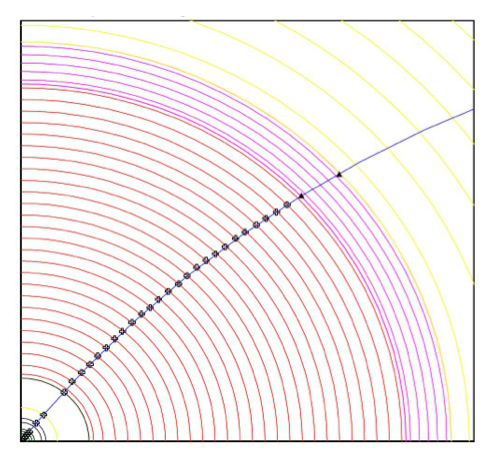
\includegraphics[width=0.3\linewidth]{chap6/fig_SGV/Tracking_SGV.png}
  \caption{Tracking in SGV \cite{Berggren2012}. The tracker is represented by pseudo-layers at which intersection with a track, the covariance matrix is calculated, going from the outer part of the tracker to the inner part (inversed Kalman filter).}
  \label{fig:tracking_sgv}
\end{figure}

In SGV, there is no definition of hits. The helix is followed through the detector to find which pseudo-layers are hit by the particle as shown in figure \ref{fig:tracking_sgv}. The tracking is done until the intersection of the start of the innermost calorimeter is reached. At each intersected pseudo-layers, the covariance matrix of the track is calculated. The covariance matrix is then translated along the particle trajectory and multiple scattering effects are included into the calculation.

In basic, it is what a Kalman filter \cite{Li2013} is doing but not in the formal way. The track fitted is matched to the vertex and the perigee parameters are then smeared according to the calculated covariance matrix. The tracking efficiency is parametrised from the full simulation.

\subsection{Calorimeter Simulation}

For the calorimeter simulation, the particle is extrapolated to the intersections with the calorimeters. At this point, a decision is made:

\begin{itemize}
  \item It is detected as a Minimum Ionising Particle (MIP).
  \item It initiates an electromagnetic shower or a hadronic shower.
  \item It is below the detector threshold.
\end{itemize}

According to the decision, the detector response is simulated from different parameters i.e. energy, type of particle, detector region\ldots\ Some parameters are controlled by steering files. Calorimeter showers can be merged if they are close to each others. To go towards more realism, the simulation of confusion between clusters can be done (Particle Flow parametrisation).

\subsection{SGV Particle Flow parametrisation}

In SGV, usual errors are already implemented i.e on detected energy, shower position and shape. However, there are association errors. Clusters might be merged, split or get associated to the wrong track.

If (a part of) a neutral cluster is wrongly associated to a charged track (so then considered as a charged cluster), energy is then lost as shown in figure \ref{fig:asso_errors}. On the other hand, if (a part of) a charged cluster is not associated to any track (considered then as a neutral cluster), the energy is double counted as shown in figure \ref{fig:asso_errors2}. Theses mis-associations give rise to an error on the total energy of an event and the particle momentum \cite{Chera2014}.

\begin{figure}[t]
  \centering
  \begin{subfigure}[t]{0.45\textwidth}
    \centering
    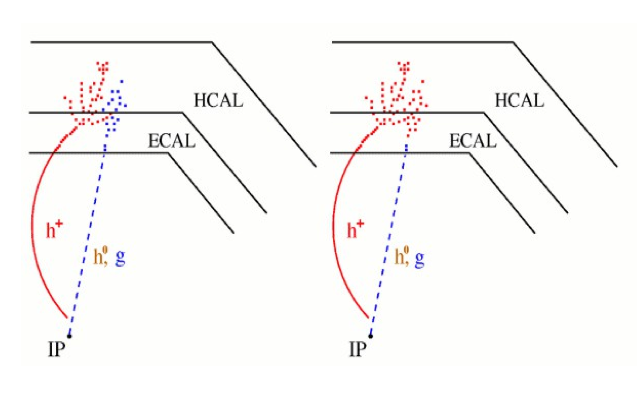
\includegraphics[width=1\linewidth]{chap6/fig_SGV/cluster_merge.png}
    \caption{Merging case.} \label{fig:asso_errors}
  \end{subfigure}
  \hfill
  \begin{subfigure}[t]{0.45\textwidth}
    \centering
    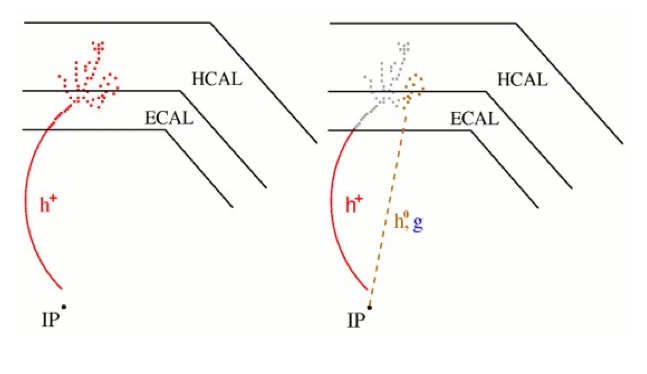
\includegraphics[width=1\linewidth]{chap6/fig_SGV/cluster_split.png}
    \caption{Splitting case.} \label{fig:asso_errors2}
  \end{subfigure}
  \caption{\subref{fig:asso_errors}) If the cluster is merged, energy is lost. \subref{fig:asso_errors2}) If the cluster is split, energy is double-counted.}
\end{figure}

The study of these association errors was done by using the Letter of Intent (LOI) mass produced samples from full simulation using the particle flow algorithm PandoraPFA  \cite{Marshall2013}. The most relevant observables were identified as: the cluster energy, the distance of the nearest particle of \"the other type\" (i.e. neutral-to-charged or charged-to-neutral), whether the particle was a hadron or not, and whether it would be detected in the barrel or endcap calorimeters. The confusion was factorized in 4 sub-processes \cite{Berggren2012}:

\begin{itemize}
  \item The probability of a cluster to split or merge as seen in figure \ref{fig:proba_split}.
  \item In case of splitting, a probability to split off/merge the \textbf{entire} cluster.
  \item In case of splitting but not completely, a function of the fraction of split off.
\end{itemize}

From this, probability distribution functions are derived (figures \ref{fig:proba_para} and \ref{fig:proba_para2}). The algorithm is applied in the Particle Flow parametrisation of SGV. So far, the results seems to be in a good agreement mostly for the neutrals but still some development is needed to get the best agreement possible between SGV and the full simulation.

\begin{figure}[t]
  \centering
  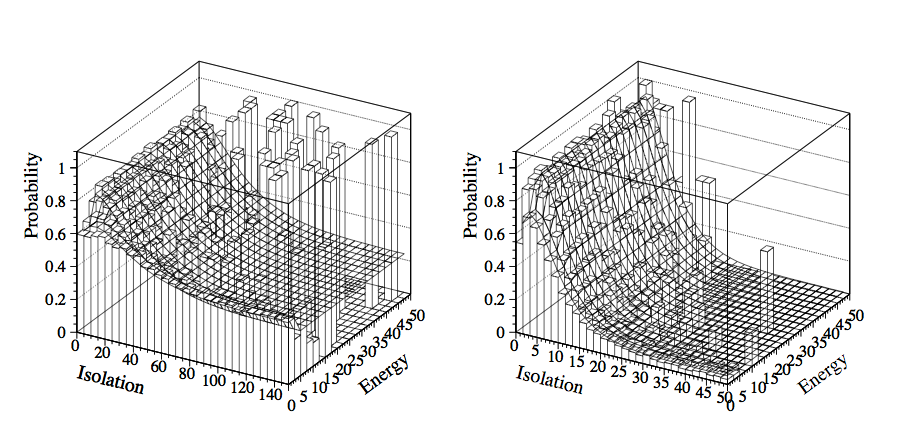
\includegraphics[width=1\linewidth]{chap6/fig_SGV/prob_split.png}
  \caption{Probability distribution of splitting in function of the cluster energy and the type of the particle.}
  \label{fig:proba_split}
\end{figure}

\begin{figure}[t]
  \centering
  \begin{subfigure}[t]{0.45\textwidth}
    \centering
    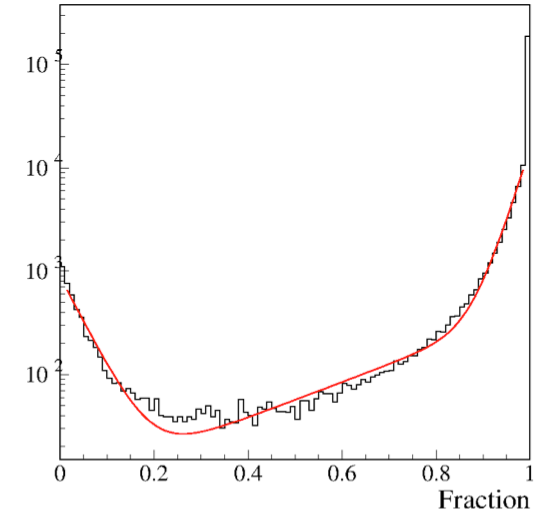
\includegraphics[width=1\linewidth]{chap6/fig_SGV/photon_loss_para.png}
    \caption{Fitting of the probability of merging for photons.} \label{fig:proba_para}
  \end{subfigure}
  \hfill
  \begin{subfigure}[t]{0.45\textwidth}
    \centering
    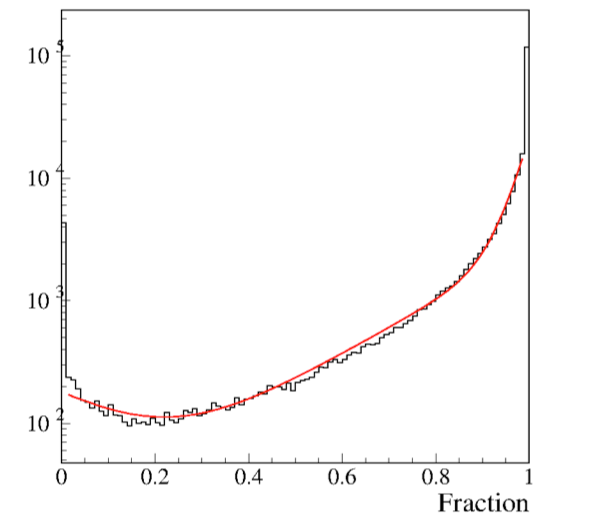
\includegraphics[width=1\linewidth]{chap6/fig_SGV/had_cha_dc_para.png}
    \caption{Fitting of the probability of splitting for charged hadrons.} \label{fig:proba_para2}
  \end{subfigure}
  \caption{\subref{fig:proba_para}) . \subref{fig:proba_para2}) .}
\end{figure}

\section{Benchmarking of fast simulation}

\subsection{Event Preparation}

The following study was perform on a simulated data sample from the Detailed Baseline Report (DBD) of \ee \ra\ \WWqqqq{} at 500 \GeV center of mass energy as shown on figure \ref{fig:DiagWWqqqq}. It is particularly interesting in order to evaluate the separation between the two $W$ bosons and the full hadronic decay complicating the reconstruction. This sample includes a \gam\gam \ra\ $hadrons$ background overlay. Several preparatory steps are performed during the reconstruction. First, a procedure is done to remove the overlay. Then hits are clustered into jets.
%%% Feyman diagram process %%%%%%%%%%%%
\begin{figure}[t]
  \centering
  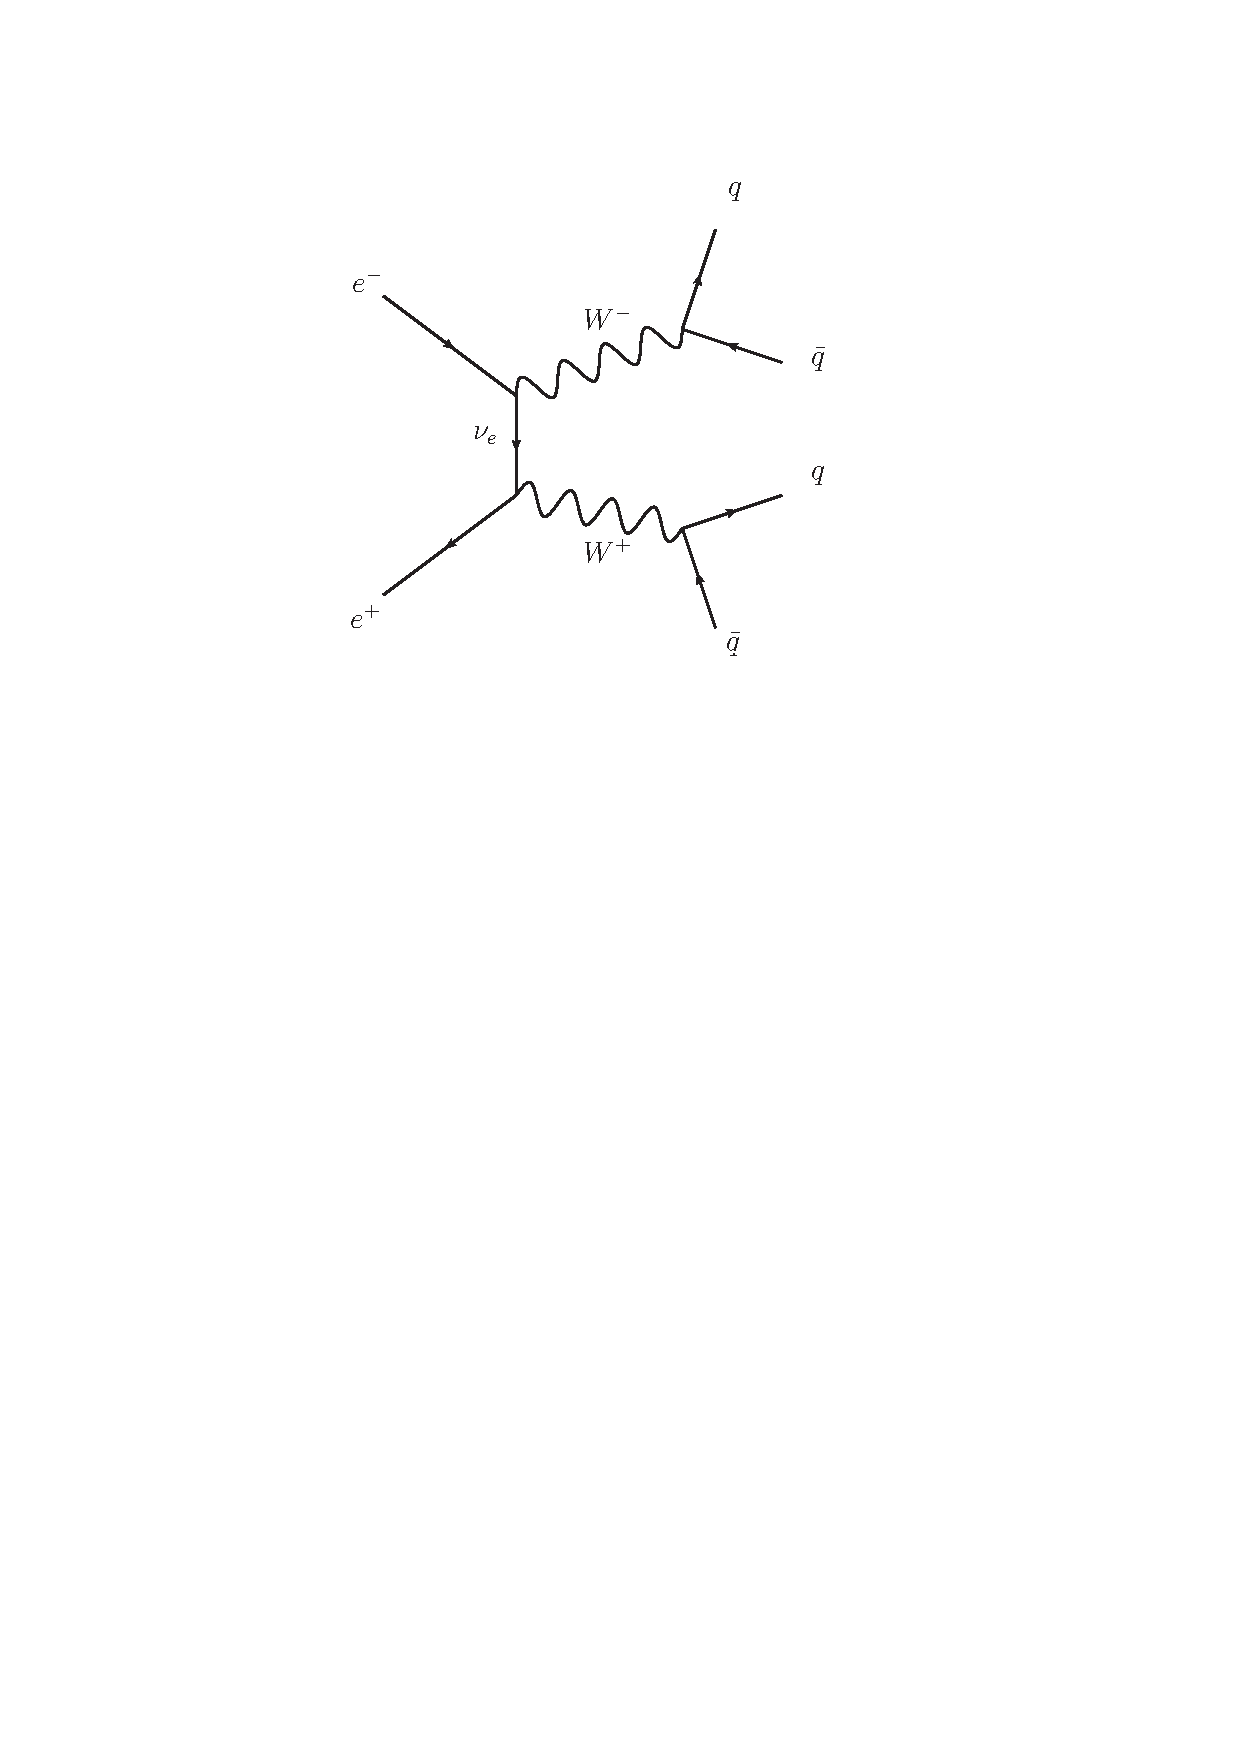
\includegraphics[trim={0 18cm 0 3cm},clip, width=1\linewidth]{chap6/fig_SGV/FeymanDiagram/DiagWWqqqq.pdf}
  \caption{Tree level Feymann diagram for the process \ee \ra\ \WWqqqq{} at \rts\ = 500 \GeV.}
  \label{fig:DiagWWqqqq}
\end{figure}

\subsubsection{Jet finding}

%% FastJet
In the final state of the process \ee \ra\ \WWqqqq{}, there are four primary quarks. These quarks will fragment and hadronise to form hadronic jets. Moreover, background such as \gam\gam \ra\ $hadrons$ may deteriorate the jet energy resolution. Thus, jet finding is very important in the event preparation.

A jet finding package called \textsc{SatoruJetFinder}\xspace was used as part of the \textsc{MarlinReco}\xspace package available in \ilcsoft. The jet finder uses an algorithm called Durham \cite{CATANI1991432, Moretti1998}. This algorithm is based on \textsc{JADE}\xspace algorithm. It utilizes a binary joining scheme by computing the distance $d_{ij}$ between two clusters $i$ and $j$ as:
\begin{equation}
  d_{ij} = 2min(E_i, E_j)(1 - cos\theta_{ij})
\end{equation}
where $E_{i,j}$ is the energy of cluster $i,j$ and $\theta_{ij}$ is the opening angle between the momentum vectors of the clusters $i,j$. If $d_{ij}$ is below $d_{cut}$, the clusters are combined such as $p_k = p_i + p_j$ with $p_{i,j,k} = (E_{i,j,k}, \mathbf{p_{i,j,k}})$, commonly called the $E-scheme$. This procedure is repeated until all pair of clusters are above $d_{cut}$. The final pair is called a jet.

For this analysis, the number of jets required is 4 due to the topology of the event. Each jets are stored as a \textsc{Reconstructed Object}\xspace in \lcio. These objects include the four momenta of the jets $(E, \mathbf{p})$ as well as each individual particle properties in a jet can be accessed.

\subsubsection{\gam\gam\ overlay removal}

For this analysis, no \gam\gam\ overlay removal method was used as Monte-Carlo information can be accessed and used during the analysis as described in the next subsection \ref{}.

But commonly, a $k_T$-algorithm can be used to remove it before the jet finding procedure. The hadrons created in the interaction of photon beams are very close to the initial beams and have almost no transverse energy. Therefore, this background looks like \"jets\" along the beam line. A $k_T$-algorithm in \textit{exclusive} mode is used to detect and remove these particles. The algorithm takes the jet radius $R$ parameter (in the order of 1) and the total number of expected jets as input. The number of expected jets and two additional for the jets along the beam line is shown to work best \cite{Mueller:301339}.

\subsubsection{\textsc{LCIOtoRoot}\xspace package}

In order to perform the analysis, a final package called \textsc{LCIOtoRoot}\xspace provided by Mickael Bergreen was used. This package is categorising the \lcio Objects (PFO, Jets, Clusters\ldots) into \textsc{ROOT}\xspace user-specific classes i.e. \textit{xRoot-TrueParticles} for Monte-Carlo level particle information. Moreover, this package includes a link between Clusters, PFO, Tracks and MC particles to know for example to which MC and/or PFO particle a track belongs to.

\subsection{Tracking efficiency}

Before reconstructing particles, PandoraPFA applies a selection on the tracks that can be a candidate for a Particle Flow Object (PFO). In this selection,
PandoraPFA assumes that everything is a pion as a first guess, which is mostly true in most cases. %This is not modified after for track energy calculation%.

Particles coming from V0s as the decay of a neutral particle in flight i.e. \gam\ \ra\ \ee, kinks as the decay of a particle into another particle of the same charge with lower momentum giving a change in the curvature i.e. $\pi^+$ \ra $\mu^++\nu$ or Prongs as the decay of a $\tau$ are identified in a first place and treated separately.
Pandora PFA uses a track selection code in order to categorise them into multi parameters categories :

\begin{itemize}
  \item CanFormPFO
  \item CanFormClusterlessPFO
  \item CannotFormPFO
\end{itemize}

To perform the categorisation, PandoraPFA applies several cuts on the track. First, it checks the number of hits of the track in the tracking chamber (TPC) and the forward tracker. The number of hits in the TPC must be between 5 and 5000 hits, in the forward tracker, a number of expected hits is calculated based on the geometry of the forward tracker if the angle of the track (tan$\lambda$) is within the acceptance of the forward tracker.

Then, the algorithm checks if the track reaches the front face of the electromagnetic calorimeter. The conditions are that the radius of the outermost hit or the max z position of all hits is above a minimum radius defined by the SET layer ($R^{SET}_{min}$) or minimum z defined by the ETD layer ($Z^{ETD}_{min}$). Or if there is a sufficient number of hits in the TPC (11) or FTD (4). If the track has a low transverse momentum, meaning that the track may curl inside the inner tracker, that the cosine angle of the track is within the acceptance of the TPC. Or that the transverse momentum of the track is above the threshold $0.3 \times B \times \frac{R^{TPC}_{outer}}{2000}$.

If the track survive all these cuts, a quality check is performed on the tracks parameters: curvature ($\Omega$), impact parameter ($d_0$), z position at the point of closest approach or p.c.a ($z_0$), radius of innermost hit ($r_{min}$) and the track energy ($E_{track}$). The curvature must be different from 0, the momentum uncertainty $\frac{\sigma_p}{p}$ must be under 15\%. If the track momentum p is over 1 \GeV, the transverse momentum $p_T$ and the momentum projected on the z axis $p_Z$ must be different of 0 \GeV and finally the number of TPC or FTD hits must be over a certain value. For TPC hits, an expected number of hits is calculated based on the geometry and the track momentum and compared to the number of measured TPC hits. For FTD hits, the number must be more than 2 hits.

Once a track passes the quality checks, Pandora categorise the track on cut-based differentiation. If a track has  $d_0 <$ 50 mm, $z_0 <$ 50 mm and $r_{min} <$ $R^{TPC}_{inner}$ + \SI{50}{\milli\meter}, the track is then categorised as \textit{\textbf{CanFormPFO}}.

A second criterion is used for non-vertex tracks i.e. tracks that are not matching the primary vertex, a check on $z_{min} - z_0$ where $z_{min}$ is the z position of the first tracker hit and the $r_{min}$ of the track is done. If the track passes through the cuts, it is flagged also as \textit{\textbf{CanFormPFO}}. If a track with unmatched vertex track has $d_0 <$ 5 mm, $z_0 <$ 5 mm, $r_{min} < R^{TPC}_{inner}$ + 50 mm and the track energy $E_{track}$ is less than 5 \GeV, the track is then categorised as \textit{\textbf{CanFormClusterlessPFO}}. For obvious reasons, tracks matching these criteria can end up in the category \textit{\textbf{CanFormPFO}}. This is then disentangled later by the track-cluster matching. For tracks that are categorised as V0s, kinks or prongs, they are also flagged as \textit{\textbf{CanFormPFO}} or \textit{\textbf{CanFormClusterlessPFO}} depending on the same criteria above. All the others tracks that do not meet the criteria are then flagged \textit{\textbf{CannotFormPFO}}, theses tracks will then not form any PFO in the reconstruction.

The goal was to check if whether Pandora rejects tracks with a PFO in SGV. As in SGV, no information is provided on the state of the track at a specific point or no tracker hit information is stored, only the relevant part of the selection made by PandoraPFA was applied. After the pseudo-selection, histograms ($h_{selected}$) for each track parameter ($d_0$, $z_0$, $cos\theta$ and $p_T$) were filled. For tracks that have the flag \"inPFO\" meaning that the track was indeed used by Pandora and formed a PFO, histograms ($h_{inPFO}$) with the track parameters were also filled.

\begin{figure}[t]
  \centering
  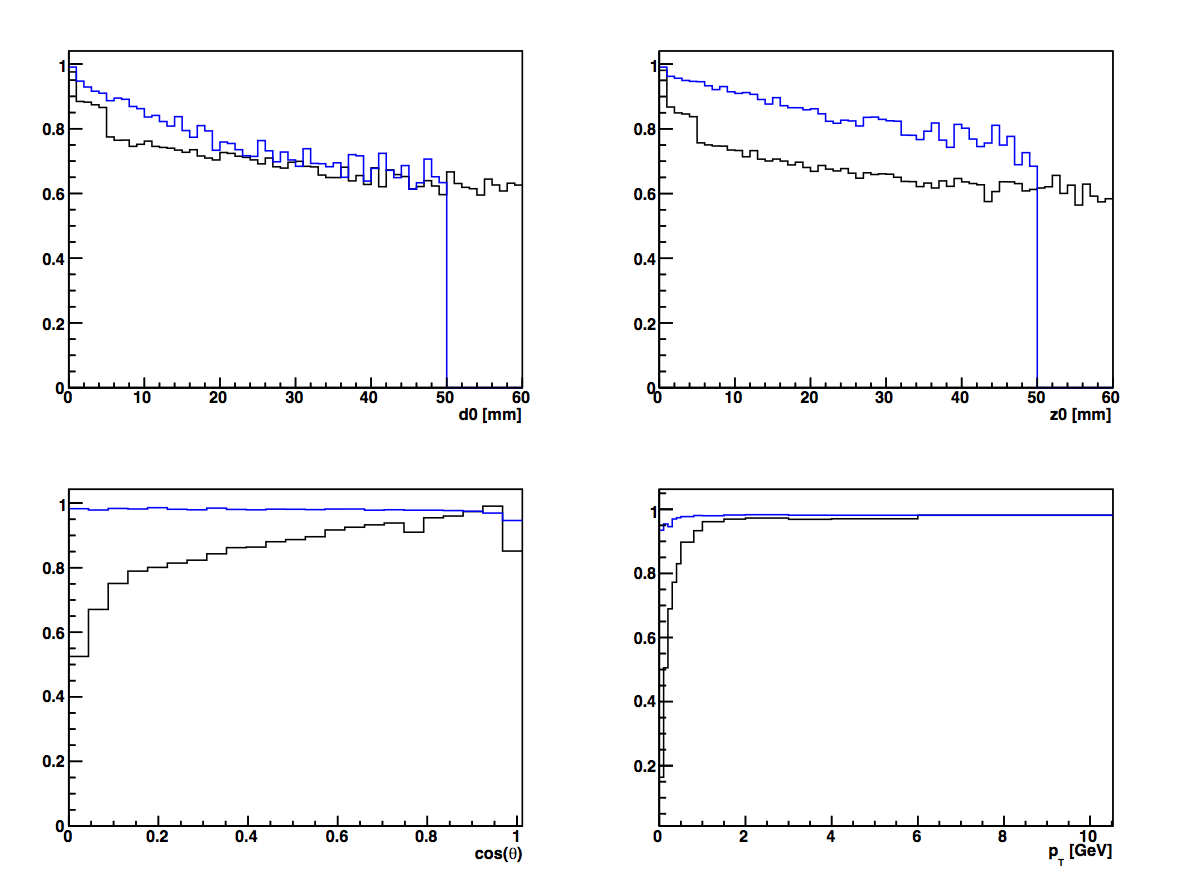
\includegraphics[width=1\linewidth]{chap6/fig_SGV/eff_track_selection_curlers.png}
  \caption{Ratio $\epsilon$ for the track parameters $d_0$, $z_0$, $cos\theta$ and $p_T$. The full simulation is represented by a black line. SGV fast simulation is represented by a blue line.}
  \label{fig:trk_select_wcurlers}
\end{figure}

To compared the performance of SGV to full simulation, a ratio $\epsilon$ was defined as $\epsilon = \frac{h_{inPFO}}{h_{selected}}$ for the full simulation. In SGV, all tracks are by default forming a PFO. With the pseudo-selection, a certain number of tracks may be rejected thus with the ratio definition above, it may be over 1. In that case, for SGV, the ratio was defined as $\epsilon = \frac{h_{selected}}{h_{inPFO}}$. The ratios for each track parameter are shown in figure \ref{fig:trk_select_wcurlers}.

As expected for the full simulation, the impact parameter ($d_0$) and the z position at the p.c.a ($z_0$) ratio plots are more or less constant. As for SGV, it seems to drop steaper but still matches quite well the full simulation. For the transverse mommentum $p_{T}$, SGV has a better ratio but this is more or less dependant on the geometry parametrisation of SGV which is relevant for low transverse momentum particles.

The main difference appears for the $cos\theta$ parameter, the full simulation seems to drop very much for very low angles compared to SGV. After further investigation, theses tracks are curlers in the TPC that make through until the endcap. At this reconstruction step, theses tracks are considered by Pandora to be able to form a PFO but further a matching between clusters and track enables to get rid of most of theses curling tracks. A cut on $z_{min} - z_0$ that should be less than half a turn of the helix can get rid of most of theses curlers as shown in figures \ref{fig:trk_para_mc_reco} and \ref{fig:trk_select_wocurlers}.

\begin{figure}[t]
  \centering
  \begin{subfigure}[t]{0.45\textwidth}
    \centering
    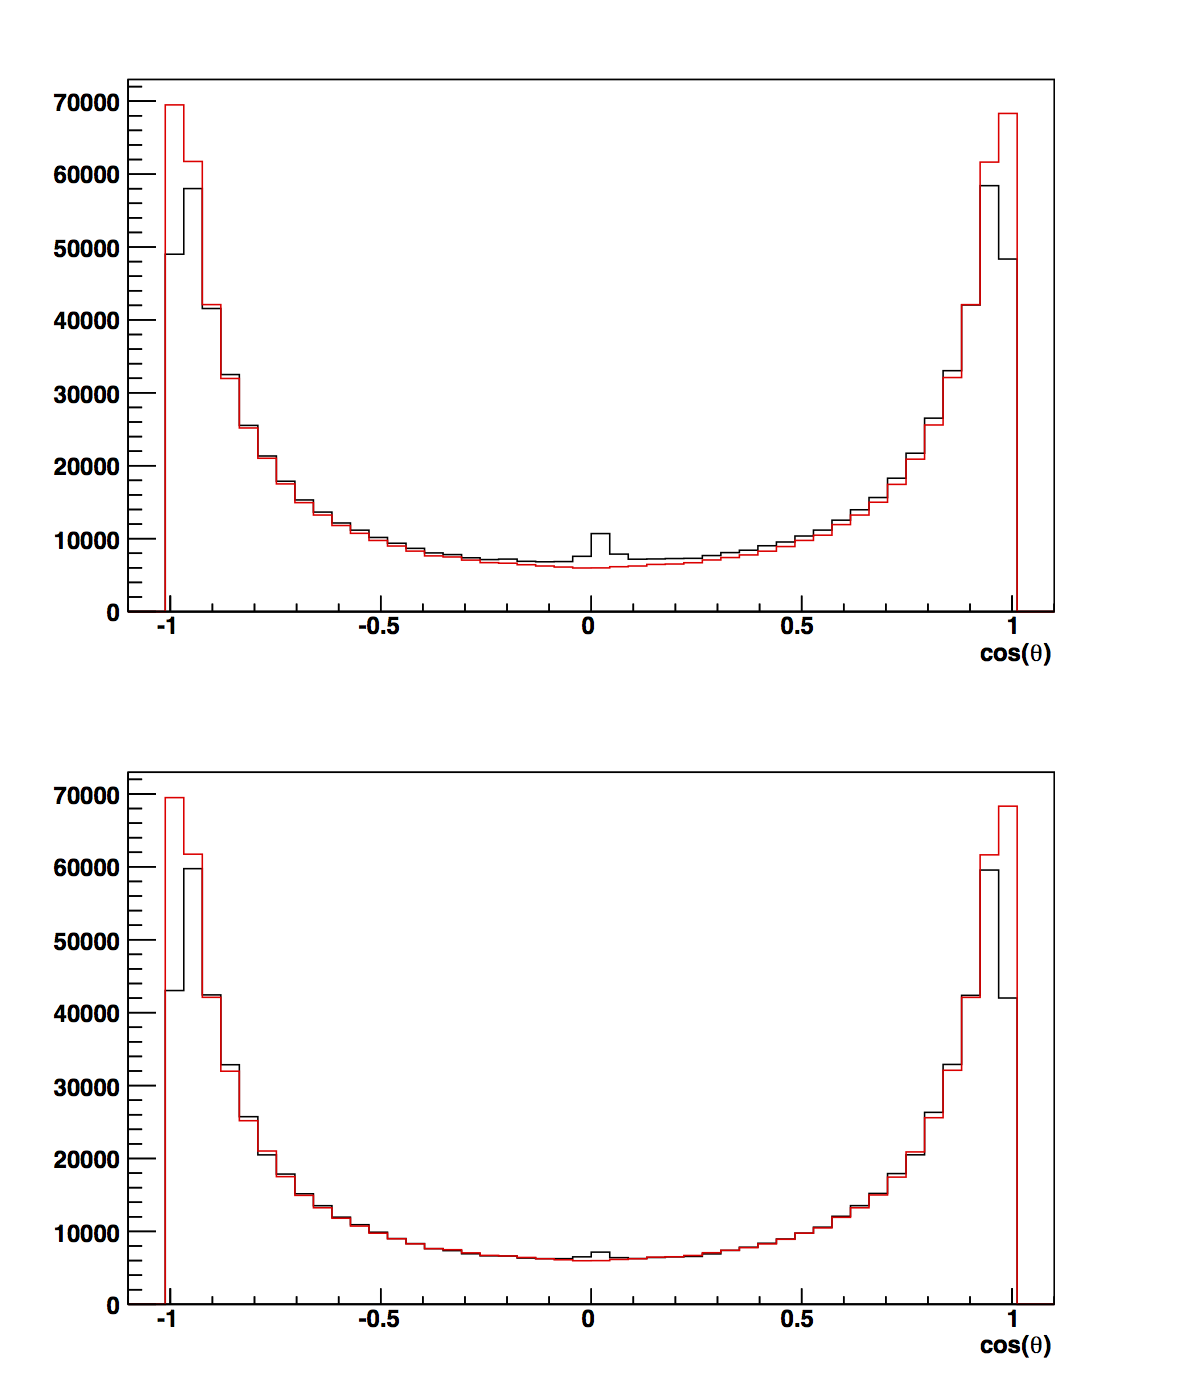
\includegraphics[width=1\linewidth]{chap6/fig_SGV/Comp_alltrk_Pandoratrk_toMC_wocurlers.png}
    \caption{$cos\theta$ distribution.} \label{fig:trk_para_mc_reco}
  \end{subfigure}
  \hfill
  \begin{subfigure}[t]{0.45\textwidth}
    \centering
    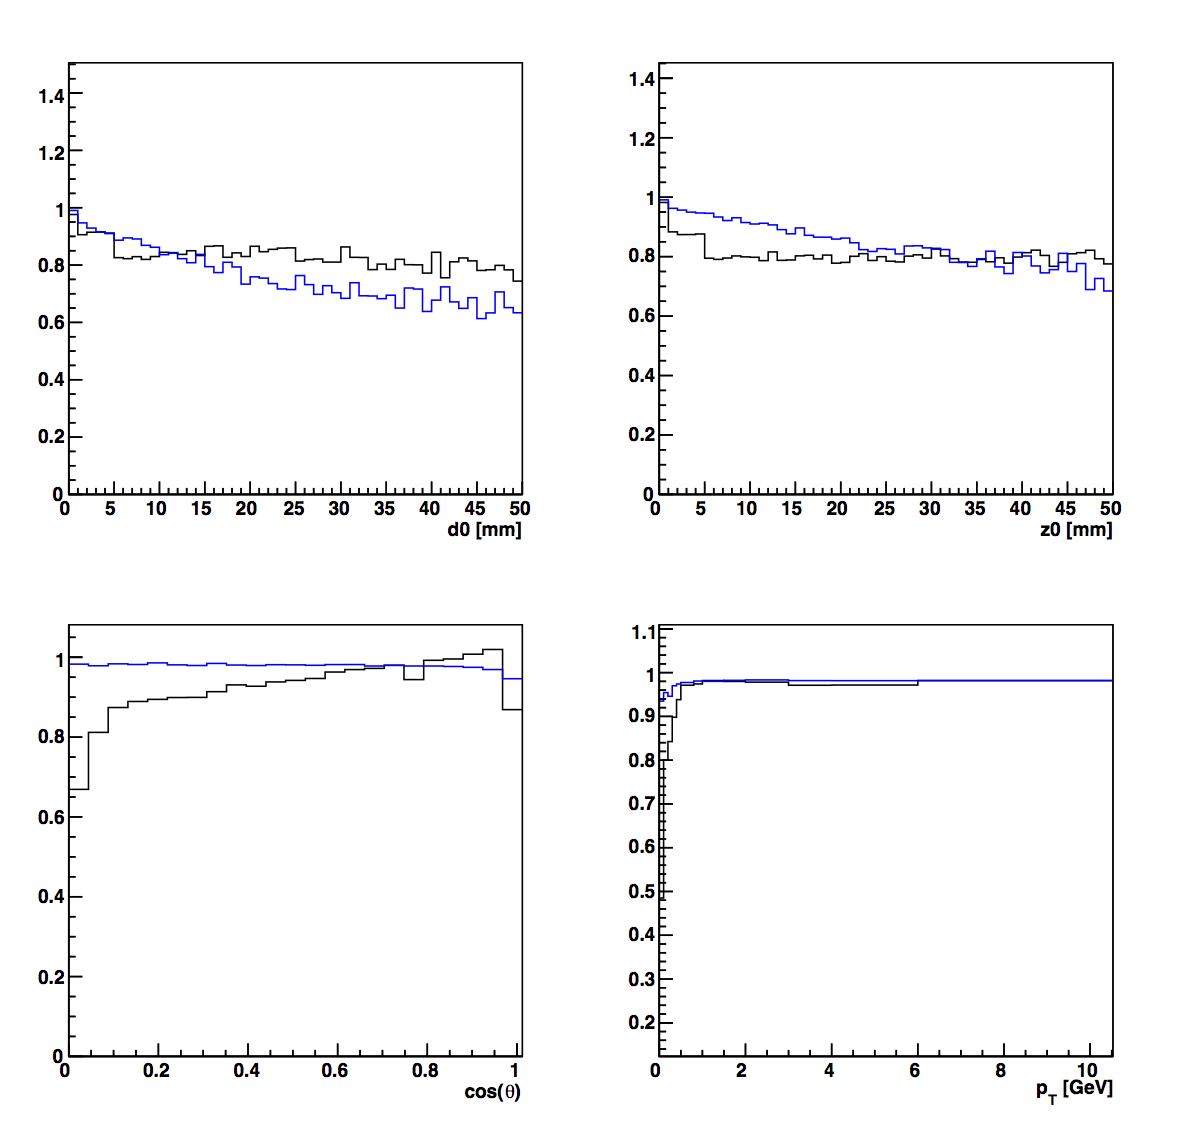
\includegraphics[width=1\linewidth]{chap6/fig_SGV/eff_track_selection_wocurlers.png}
    \caption{Ratio $\epsilon$ of the track parameters.} \label{fig:trk_select_wocurlers}
  \end{subfigure}
  \caption{\subref{fig:trk_para_mc_reco}) The top plot shows the $cos\theta$ distribution of MC tracks in red and Pandora track in blue with the pseudo-selection in SGV. The bottom plot shows the $cos\theta$ distribution of MC tracks in red and Pandora track in blue with the pseudo-selection and an additional cut on $z_{min}$ to remove curling tracks in SGV. \subref{fig:trk_select_wocurlers}) Ratio $\epsilon$ of the track parameters $d_0$, $z_0$, $cos\theta$ and $p_T$ after additional cut on curling tracks. The black line represent the full simulation and the blue line represent SGV fast simulation.}
\end{figure}

By adding this cut, SGV and the full simulation agrees better. Nevertheless, the introduced cut seems still not enough to get rid of most of the curlers looking at the $cos(\theta)$ distribution. This shows that the tracking selection in PandoraPFA is not responsible for the observed discrepancy.

\subsection{Track multiplicity and Correlation track/energy}

A look at the number of tracks or multiplicity inside a jet was performed in order to see if SGV performs as expected. The number of tracks were counted per jet energy bins for full simulation, SGV with and without the Particle Flow parametrisation as shown on figure \ref{fig:trk_multiplicity}.

\begin{figure}[t]
  \centering
  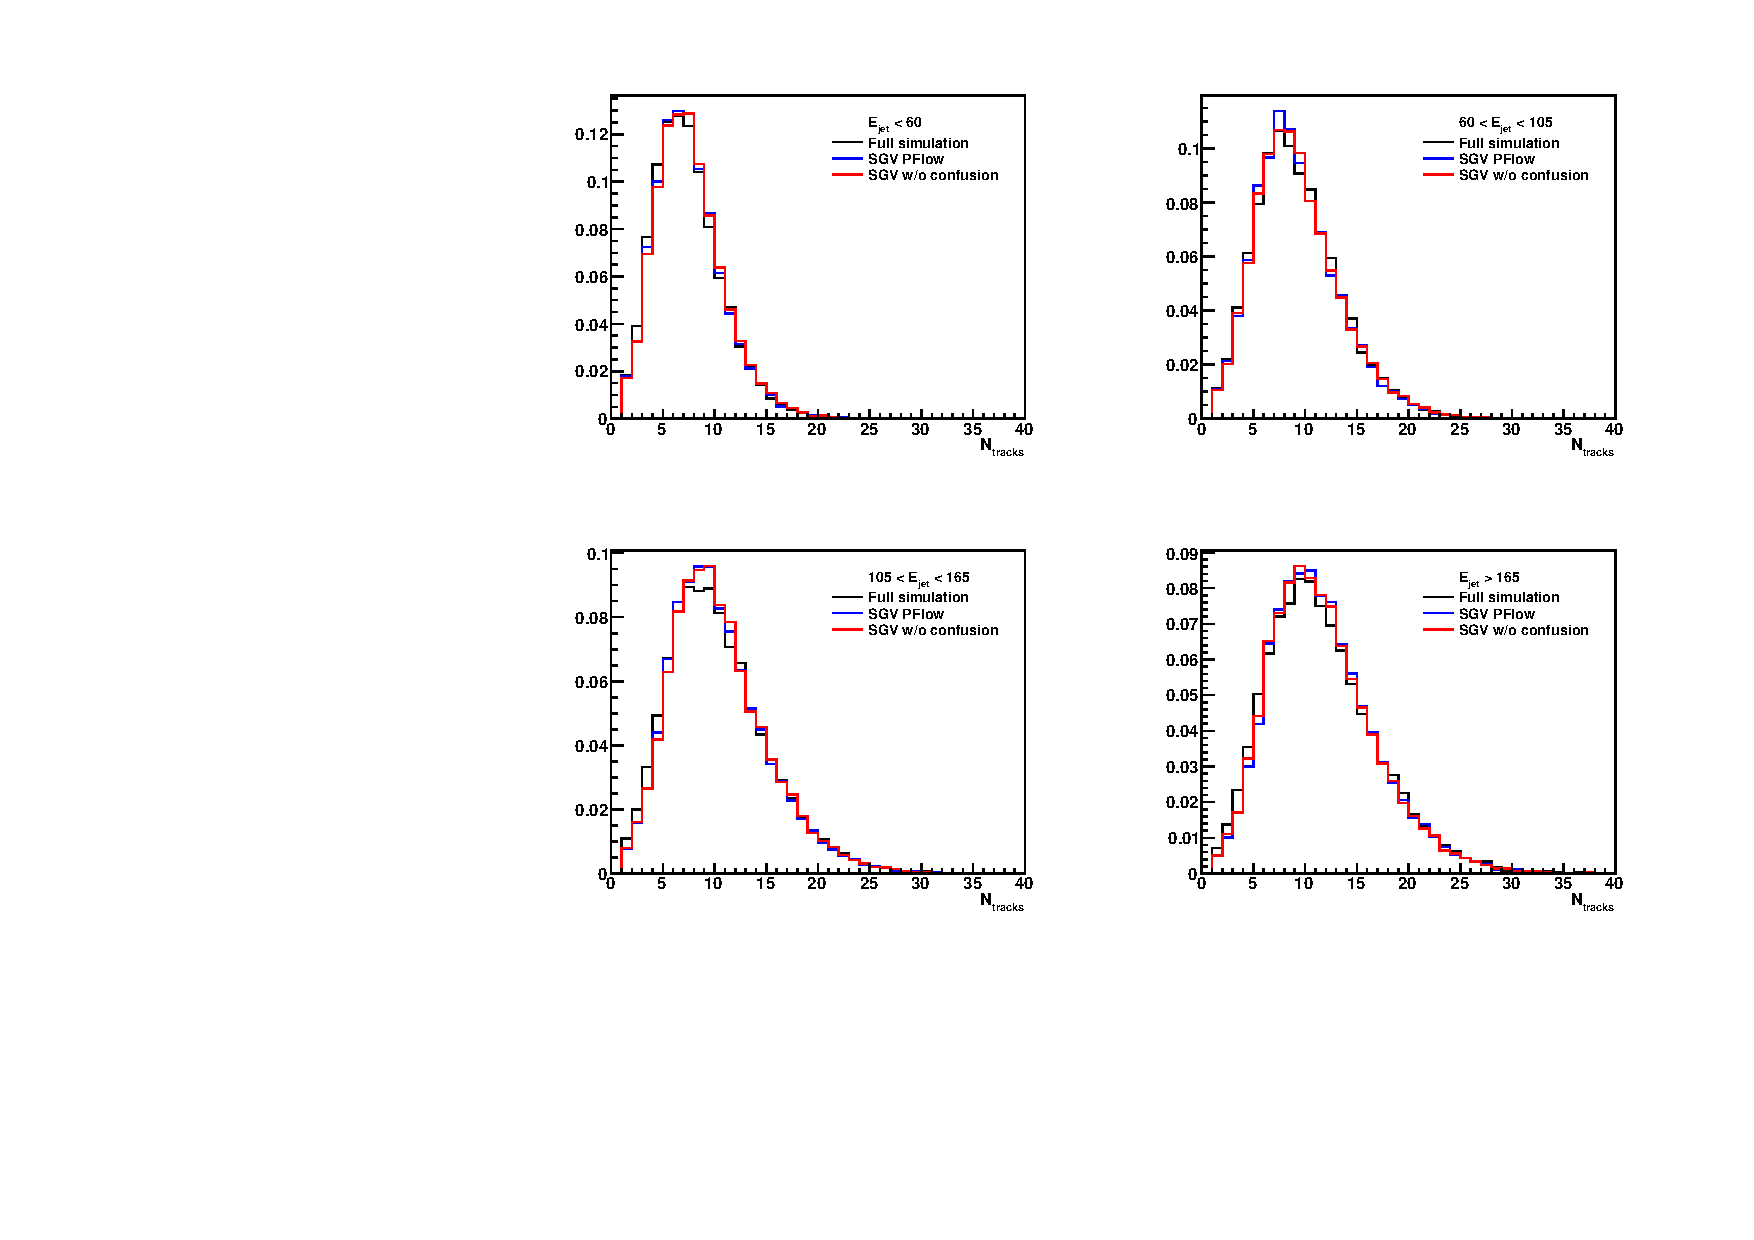
\includegraphics[width=1\linewidth]{chap6/fig_SGV/multiplicity_jet_track.pdf}
  \caption{Track Multiplicity in bins of jet energy. The full simulation is in black line, SGV without the particle flow parametrisation is in red and SGV with the parametrisation is in blue. The results in SGV are in a very good agreement with the full simulation.}
  \label{fig:trk_multiplicity}
\end{figure}

One can see that the multiplicity of tracks are in very good agreement between SGV and full simulation. Here the particle paramtrisation has a minimal impact on the pattern recognition and the association track-cluster as shown by the blue and red lines which are very similar.

Typically, jets are composed of 60-70\% of charged particles, 10\% of photons and 20-30\% of neutrals. The correlation between the fraction of charged energy in a jet and track multiplicity was also looked at. The distributions shown on figures \ref{fig:correlation_distrib_full} and \ref{fig:correlation_distrib_sgv} are in agreement and correspond to what is expected.

\begin{figure}[t]
  \centering
  \begin{subfigure}[t]{0.45\textwidth}
    \centering
    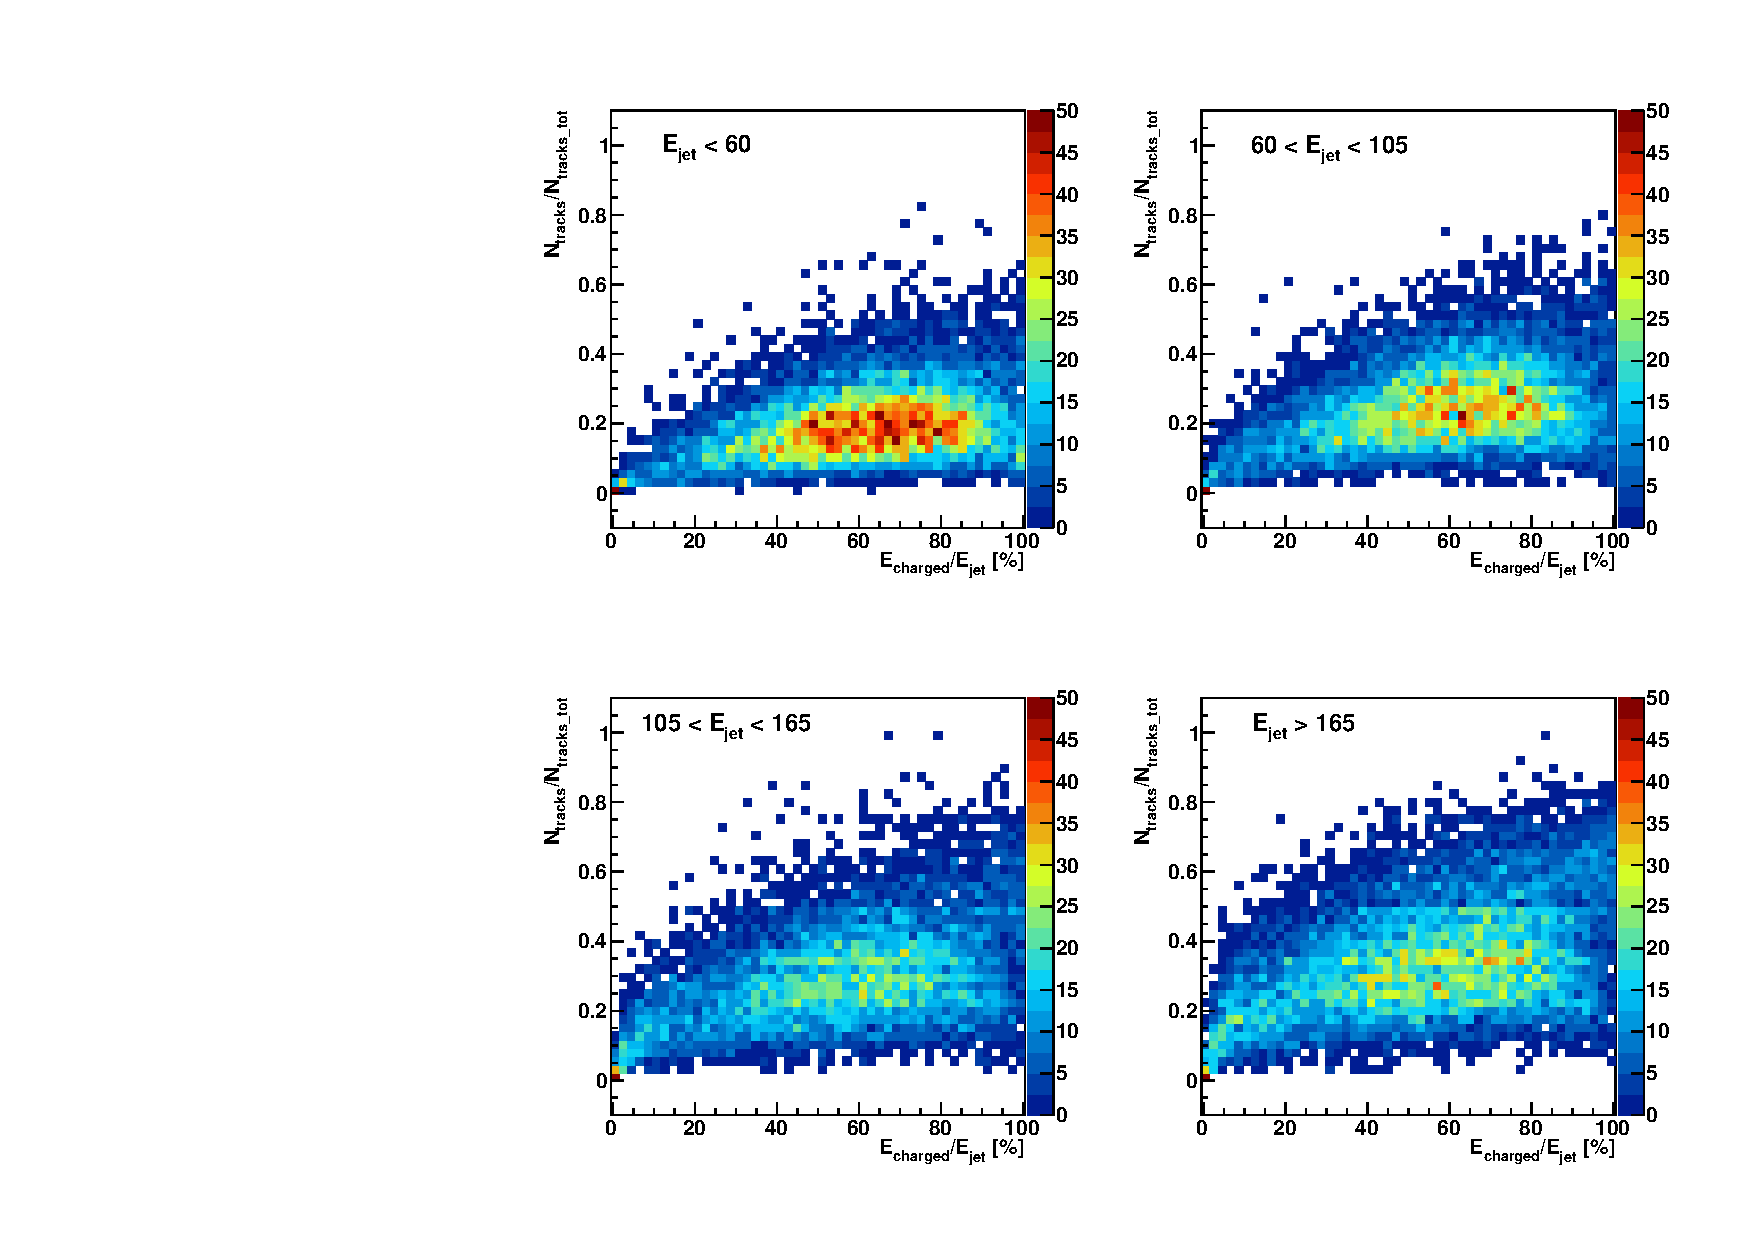
\includegraphics[width=1\linewidth]{chap6/fig_SGV/Correlation_Ntrack_FracEchajet_full.pdf}
    \caption{DBD full simulation.} \label{fig:correlation_distrib_full}
  \end{subfigure}
  \hfill
  \begin{subfigure}[t]{0.45\textwidth}
    \centering
    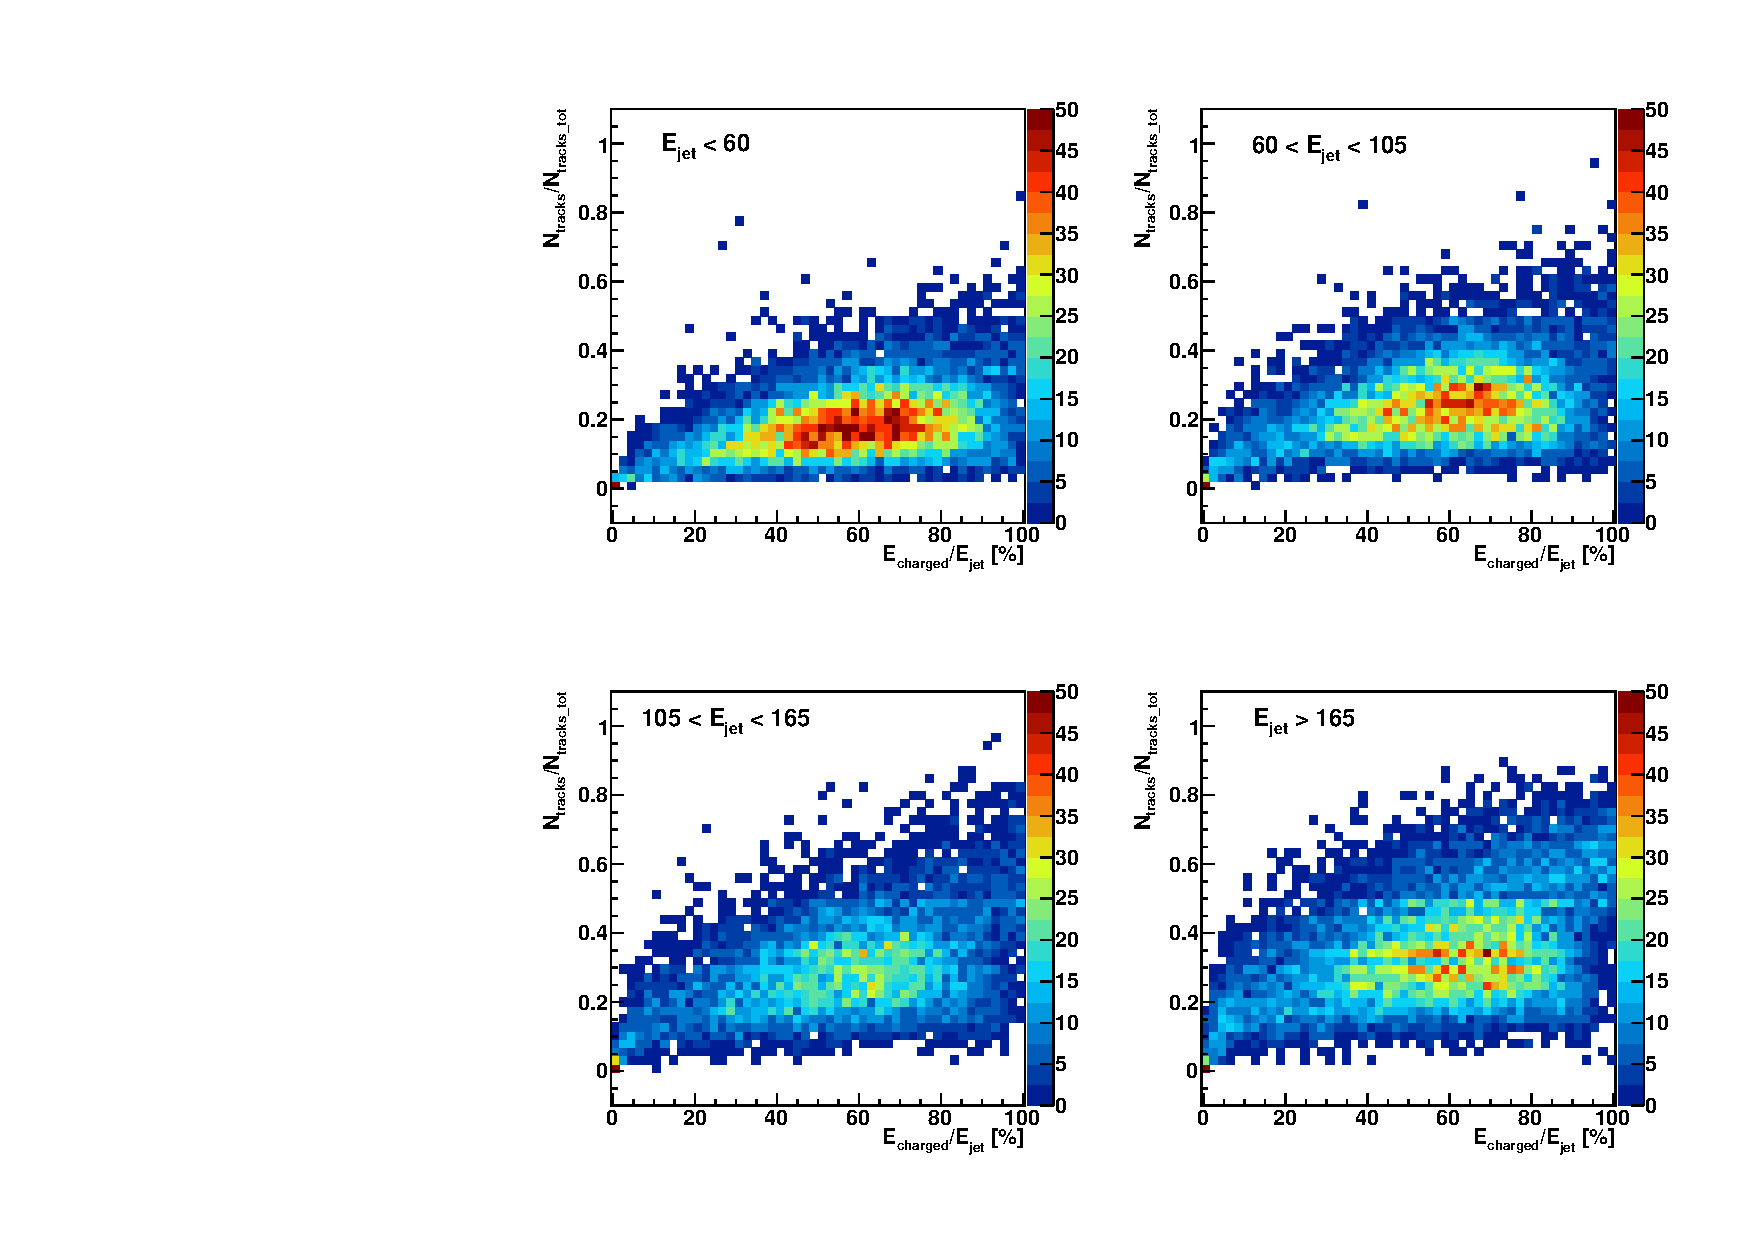
\includegraphics[width=1\linewidth]{chap6/fig_SGV/Correlation_Ntrack_FracEchajet_sgv.pdf}
    \caption{SGV fast simulation.} \label{fig:correlation_distrib_sgv}
  \end{subfigure}
  \caption{\subref{fig:correlation_distrib_full}) Correlation track multiplicity normalised to the total number of tracks versus the charged energy normalised to the jet energy for different jet energy bins for the full simulation. \subref{fig:correlation_distrib_sgv}) Correlation track multiplicity normalised to the total number of tracks versus the charged energy normalised to the jet energy for different jet energy bins for SGV.}
\end{figure}

\section{Particle Flow studies}

\subsection{Double counted and lost energy}

Association errors can happen during reconstruction as explained in section \ref{} because of a confusion term coming from the overlap of showers into the calorimeters.

\begin{figure}[t]
  \centering
  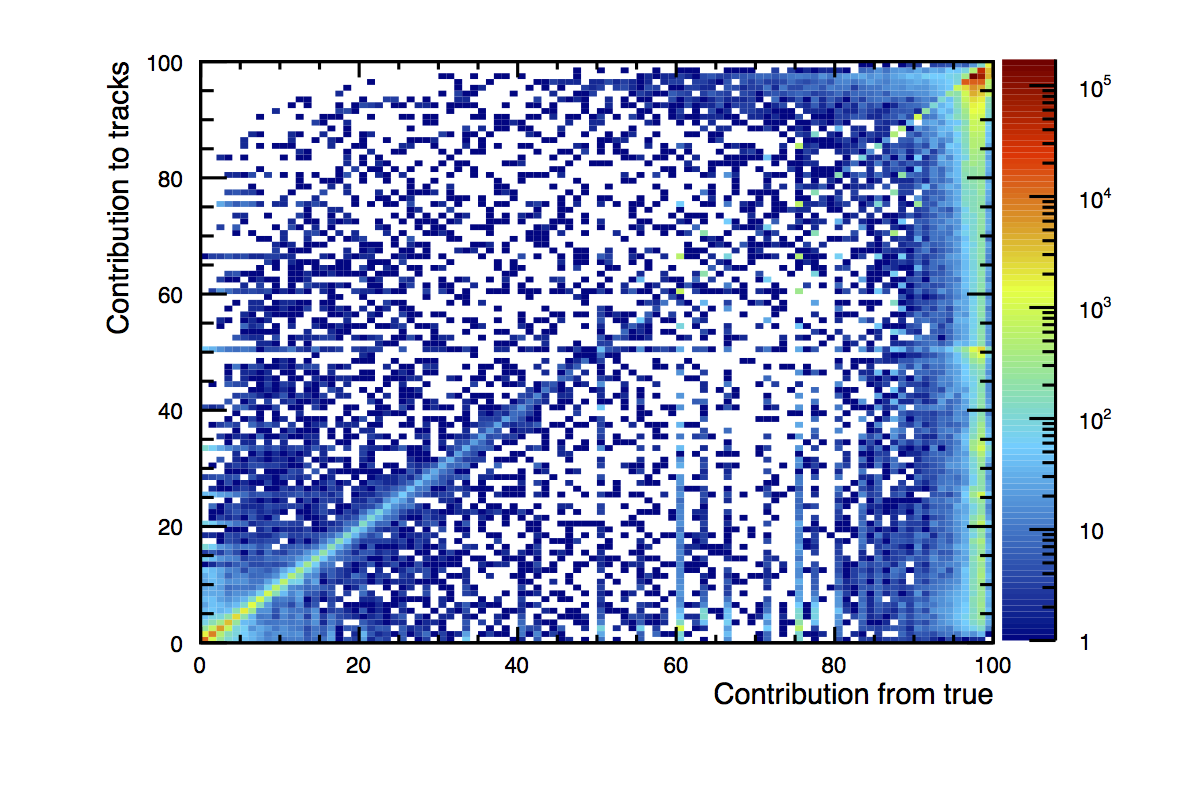
\includegraphics[width=1\linewidth]{chap6/fig_SGV/weight_corr.png}
  \caption{Distribution of the weights of track-true particle relation. The contribution from true represent the contribution of a true particle to a track in terms of hits from this true particle compared to the total hits in the track and the contribution to track represent the inverse relation, the number of hits from a true particle compared to the total of simulated hits from this true particle.}
  \label{fig:weight_tracks}
\end{figure}

The figure \ref{fig:weight_tracks} revells 2 regions, the top right corner and the bottom left corner. The top right corner represents the region where there is almost no confusion between a track and the Monte-Carlo particle associated. There is almost a one-to-one relation between a track and a true particle, i.e., one true particle is associated to a track. The bottom left corner is the region where the confusion dominates, this region shows that it is difficult to associate correctly a particle to a track, the contributions to a track seem to come from different particles.

The goal of particle flow is to avoid confusion as much as possible. There can be different points of view concerning the treatment of the double counted and lost energy:
\begin{itemize}
  \item At a cluster-track level by comparing the energy of a track (momentum + assumption of $\pi$ mass) to the energy of the cluster associated to the track (it would be then an energy flow point of view).
  \item At a jet level (clusters contained into a jet) by looking at the double counted and lost energy over the jet energy.
\end{itemize}

\subsubsection{At Cluster-Track level}

At a Cluster-Track level, the following method has been pursued. For each event, each reconstructed particle is taken, then one look at the track associated to the reconstructed particle and calculate the track energy as:
\begin{equation}
  E_{track} = \sqrt{\|\overrightarrow{p}\| \cdot \|\overrightarrow{p}\| + m_{\pi}^{2}}
\end{equation}
with $m_{\pi}$ = 0.139 \GeV and $\overrightarrow{p}$, the reconstructed particle momentum. The pion assumption is made like in PandoraPFA which in most cases is not wrong and will not affect the calculated energy by much. Then the cluster associated to the reconstructed particle is looked at and the energy of the cluster $E_{cluster}$ is taken. A comparison between the track energy $E_{track}$ and the cluster energy $E_{cluster}$ then is done.

If $E_{track} < E_{cluster}$, the difference is categorized as double-counted energy. Naturally the energy of the cluster should be the track energy because the resolution of the tracker is much better than the calorimeter. So if there is more energy in the cluster it means that a part of it may come from a near neutral particle or from a mis-measurement. If the opposite is true i.e. $E_{track} > E_{cluster}$, then it is categorized as lost energy. The double counted and lost energy is summed up for all the particles in the event. This method is done for each reconstructed particles in an event, thus for each event we have a point $E_{dc}$ and $E_{lost}$. The result is shown on figure \ref{fig:cluster_track_level}.

\begin{figure}[t]
  \centering
  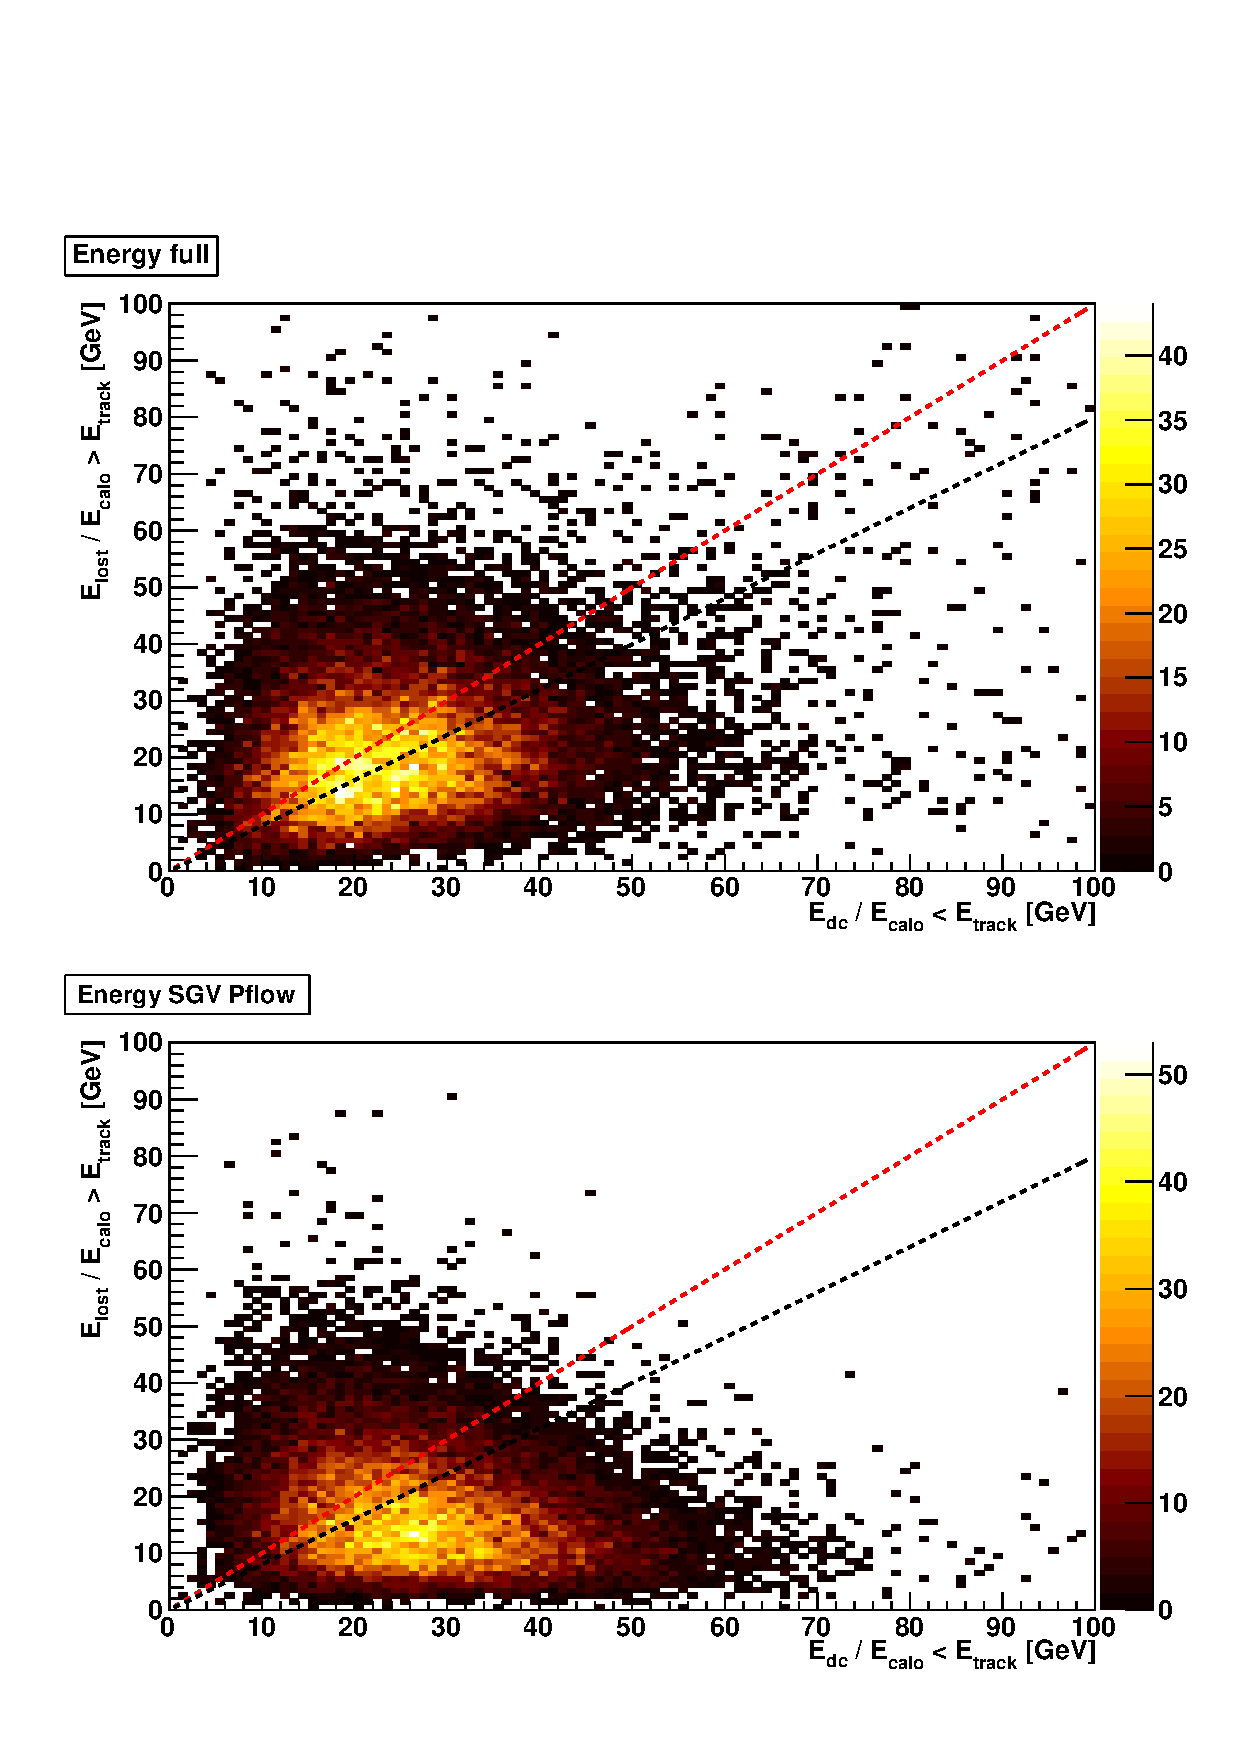
\includegraphics[width=1\linewidth]{chap6/fig_SGV/Correlation_nojet.pdf}
  \caption{2D plot representing the lost energy versus the double-counted energy. The top plot is the full simulation and the bottom plot is SGV fast simulation. Each point in this plot represents an event. The red and the black dotted line indicate a correlation of 100\% and 80\%. One can observe that there is slightly different correlations for SGV and the full simulation.}
  \label{fig:cluster_track_level}
\end{figure}

In the full simulation, it seems that PandoraPFA is leveling between the lost and double counted energy. Pandora may balancing both quantities on event by event basis. For SGV, the correlation is very similar with the parametrisation. SGV is has a tendency to have more double counting energy than lost energy indicating that SGV tends to split more clusters.

\begin{figure}[t]
  \centering
  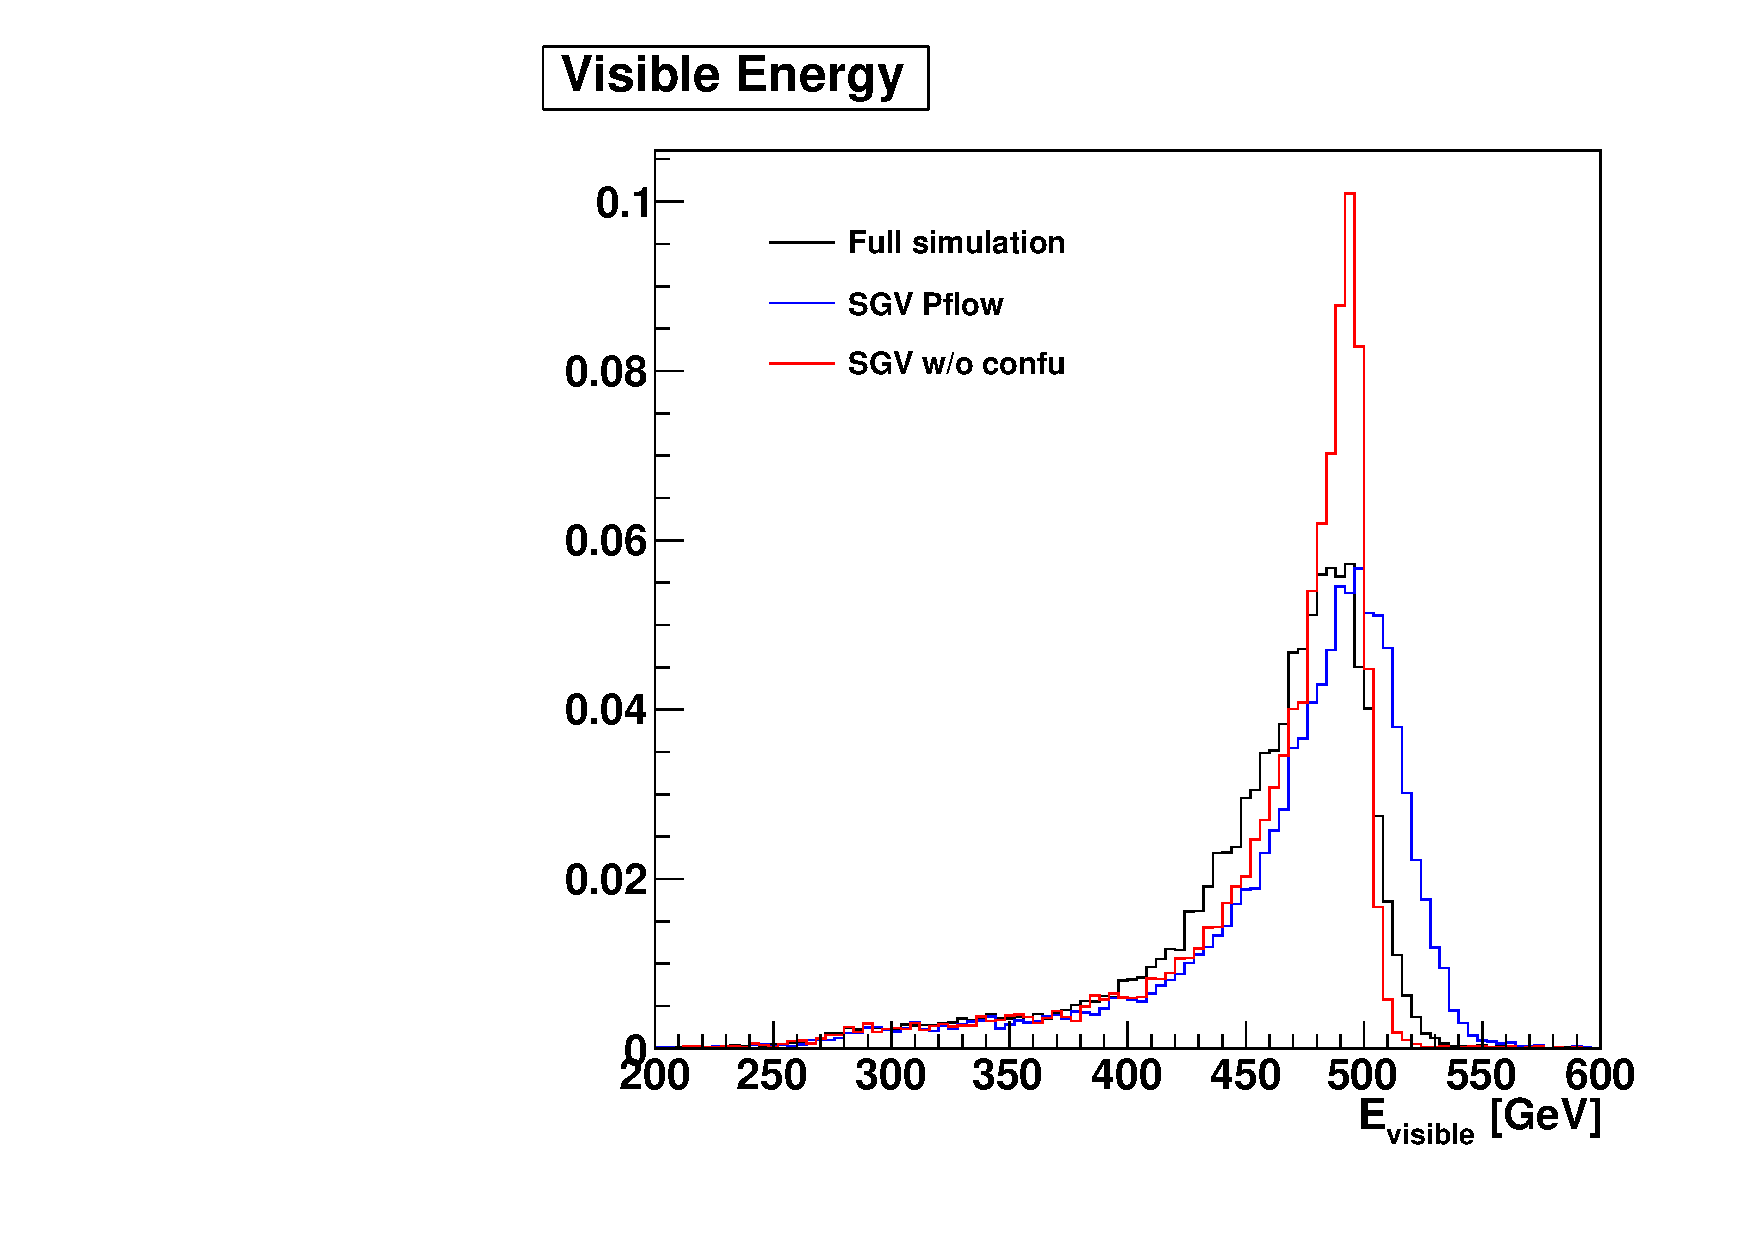
\includegraphics[width=1\linewidth]{chap6/fig_SGV/Evis.pdf}
  \caption{Representation of the total energy of all events for the full simulation in black line and SGV with (in blue line) and without the particle flow parametrisation (in red line).}
  \label{fig:energy_total}
\end{figure}

Looking at the total energy as shown on figure \ref{fig:energy_total}, SGV without the particle flow parametrisation seems to describe well the total energy but doesn't include the reconstruction effects explaining the smaller width of the distribution. When the parametrisation is used, a tail in the total energy appears. Though the width of the distribution seems correct, a shift in energy is visible. Therefore, the energy distribution of neutral and charged reconstructed particles was looked at as shown on figure \ref{fig:energy_charged_neutral}.

\begin{figure}[t]
  \centering
  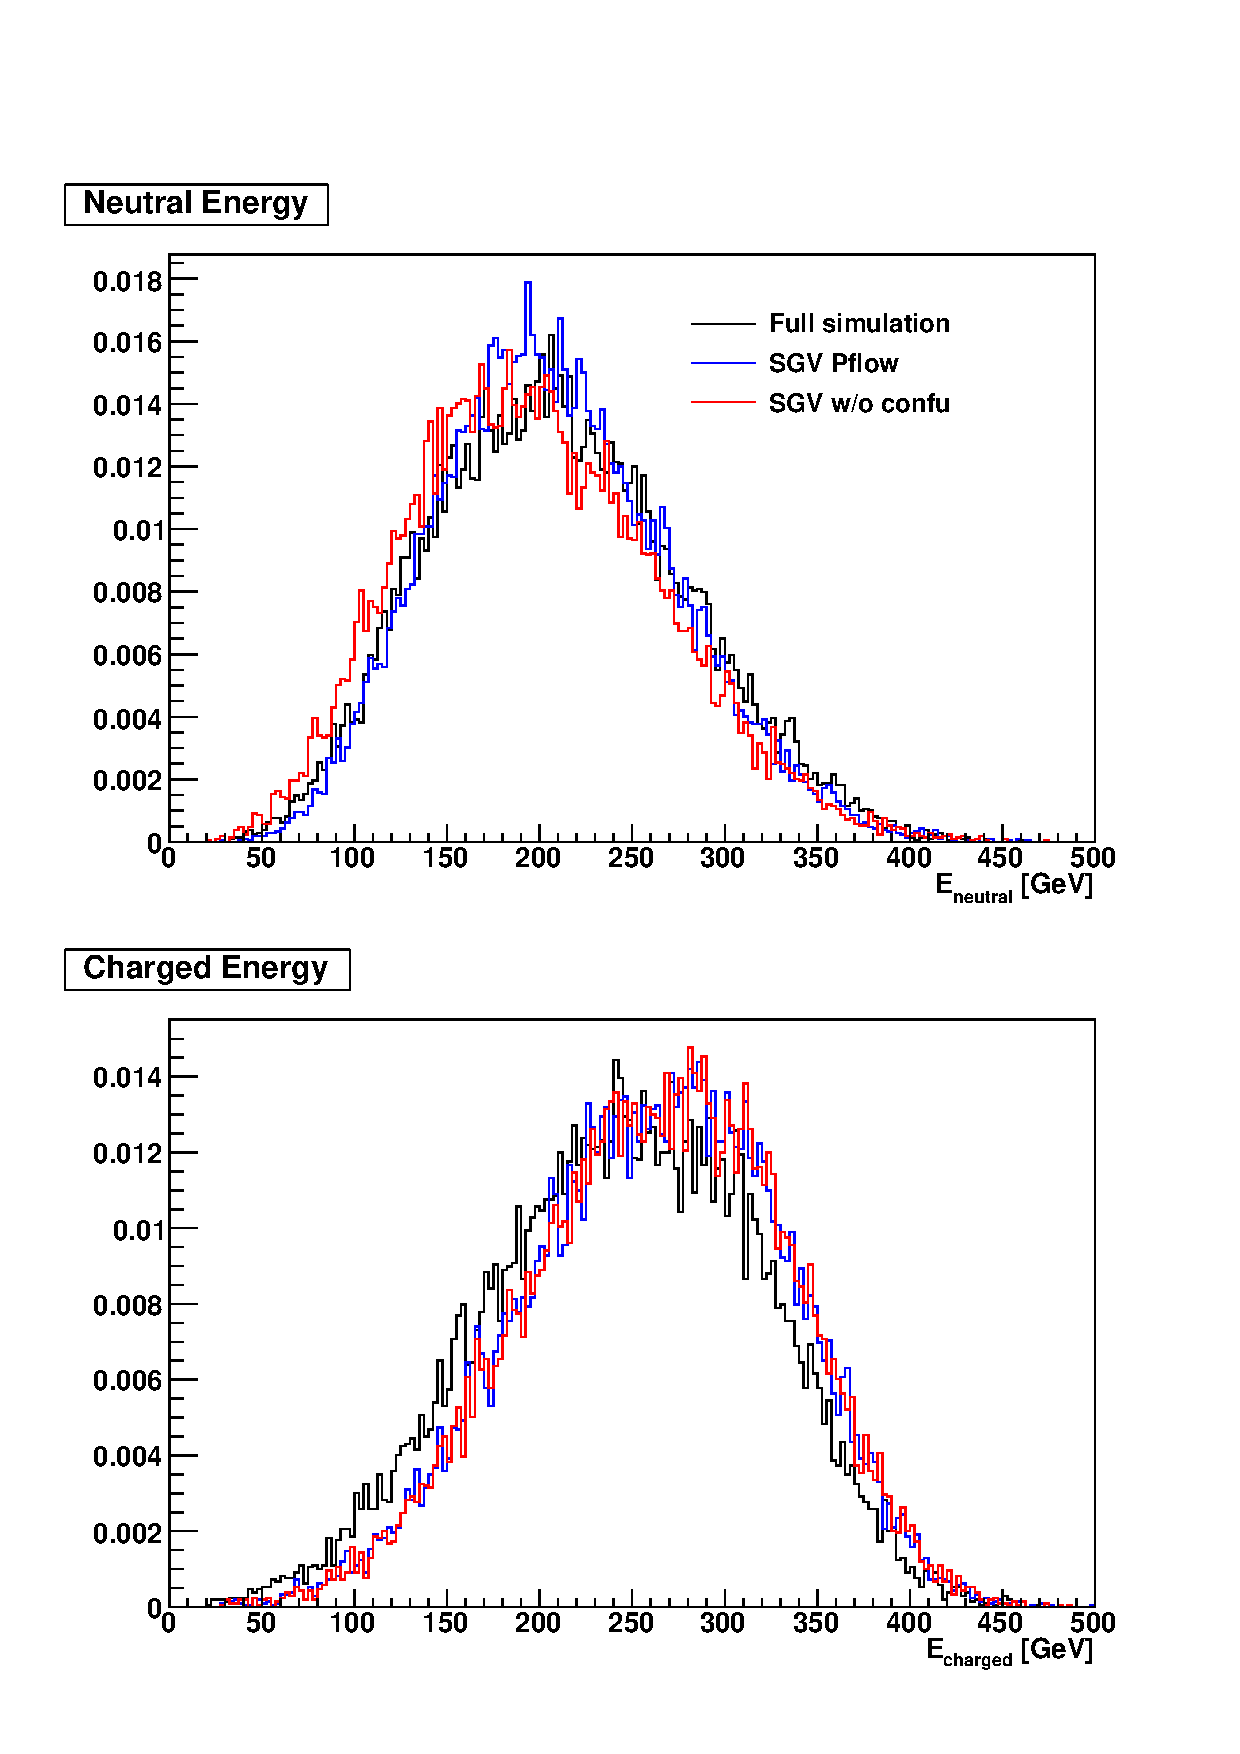
\includegraphics[width=1\linewidth]{chap6/fig_SGV/Total_EneuEcha_notjet.pdf}
  \caption{The top plot represents the total charged reconstructed particle energy. The bottom plot represents the total neutral reconstructed particle energy. SGV is indicated by a blue line (red line) with the particle flow parametrisation (without respectively) and the full simulation in black line.}
  \label{fig:energy_charged_neutral}
\end{figure}

The neutral energy distribution improves in SGV with the particle flow parametrisation and agrees well with the full simulation. But for the charged energy, the parametrisation doesn't change anything. This is expected because only the track information matters in this case and not the cluster in the calorimeters. The distribution is shifted to higher energies explaining the tail observed in the total energy distribution. This gives a hint that the parametrisation should have an effect on the charged particles. Which can be possible in the case that the track information is rejected (i.e. due to a bad track fitting) and only the calorimeter information is taken into account. Therefore, the same quantities were looked at the jet energy level in order to see at what energy scale the discrepancy appears.

\subsubsection{At Jet level}

The process \ee \ra\ \WWqqqq{} at \rts\ = 500 \GeV has a typical topology of 4 jets from the 4 primary quarks. The jets are obtained by running the Durham algorithm after the reconstruction. The Durham algorithm is a $k_T$-algorithm, it clusters all reconstructed particles into jets as explained in section \ref{}.

\begin{figure}[t]
  \centering
  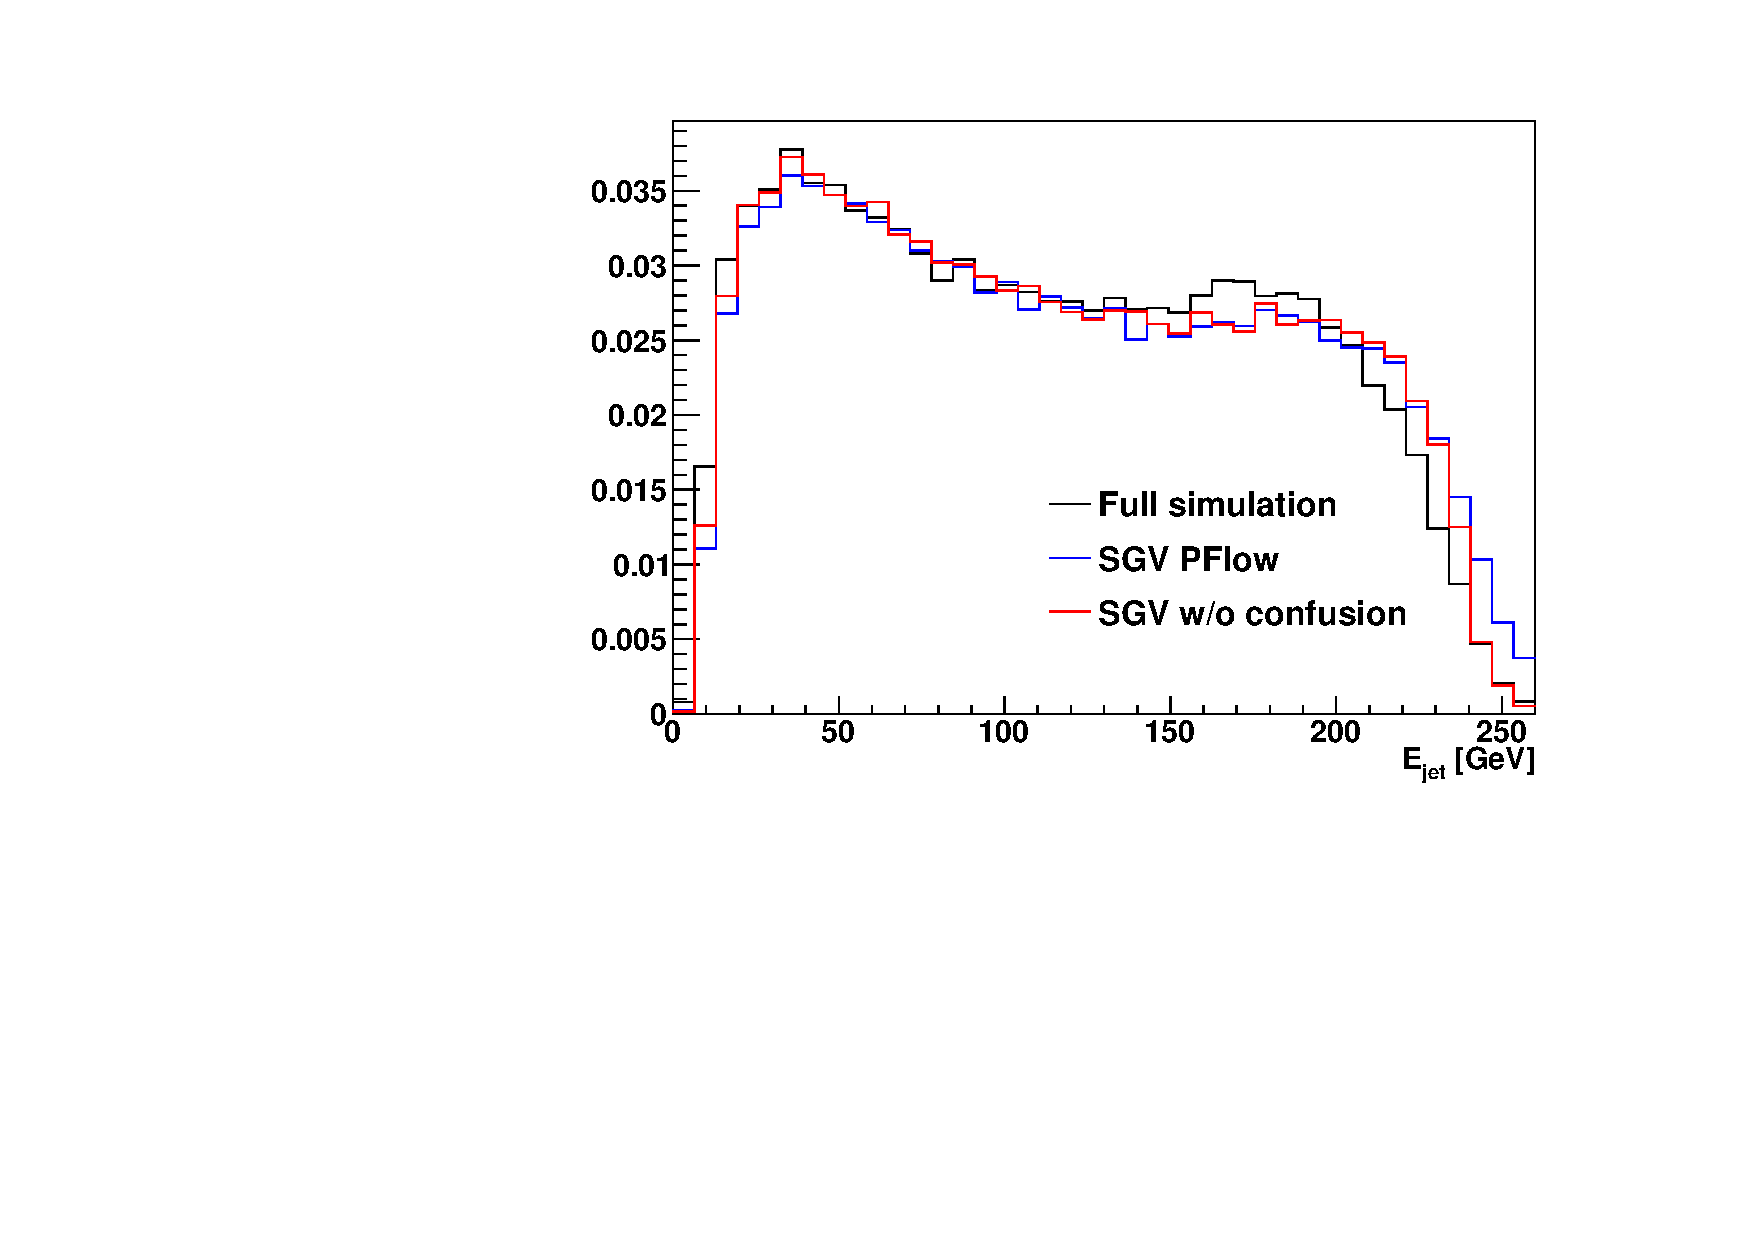
\includegraphics[width=1\linewidth]{chap6/fig_SGV/Jet_spectrum.pdf}
  \caption{Jet energy spectrum between the full simulation in black line and SGV in blue (red) line with (without) the particle flow parametrisation.}
  \label{fig:jet_spectrum}
\end{figure}

First, jets are classified into few energy bins for each event: 0 to 60 \GeV, 60 to 105 \GeV, 105 to 165 \GeV and over 165 \GeV. The energy bins were selected in order to have the same order of number of events per jet energy bin as seen on figure \ref{fig:jet_spectrum}. Then, inside each jet, each reconstructed particle is taken. The same method as the section above is used. Now, $E_{lost}$ and $E_{dc}$ were calculated per jet. At the end, the lost energy versus the double-counted energy are normalised to the jet energy as shown on figures \ref{fig:jet_track_level_full} and \ref{fig:jet_track_level_sgv}.

For low jet energies, SGV and the full simulation seems to be in agreement. On the other hand, the higher the jet energy is, the more differences become visible. For jet energies over 165 \GeV, SGV is double-counting much more than the full simulation which stays with a good correlation between $E_{dc}$ and $E_{lost}$. This gives an indication that SGV is failing in regions where jet energies are high, over 165 \GeV.

The reason could be that, in these cases, the energy density in the calorimeter is so high. So that the association errors can be committed more easily because the confusion term of the overlapping showers is getting bigger and bigger in function of the jet energy. PandoraPFA, to solve this problem, may be switching to a pure \"Energy Flow\" mode. Meaning that it is discarding the track information and only keeps the calorimeter information. And by reclustering, PandoraPFA is matching the overall energy in a calorimeter region to the tracks in the same region.

\begin{figure}[t]
  \centering
  \begin{subfigure}[t]{0.45\textwidth}
    \centering
    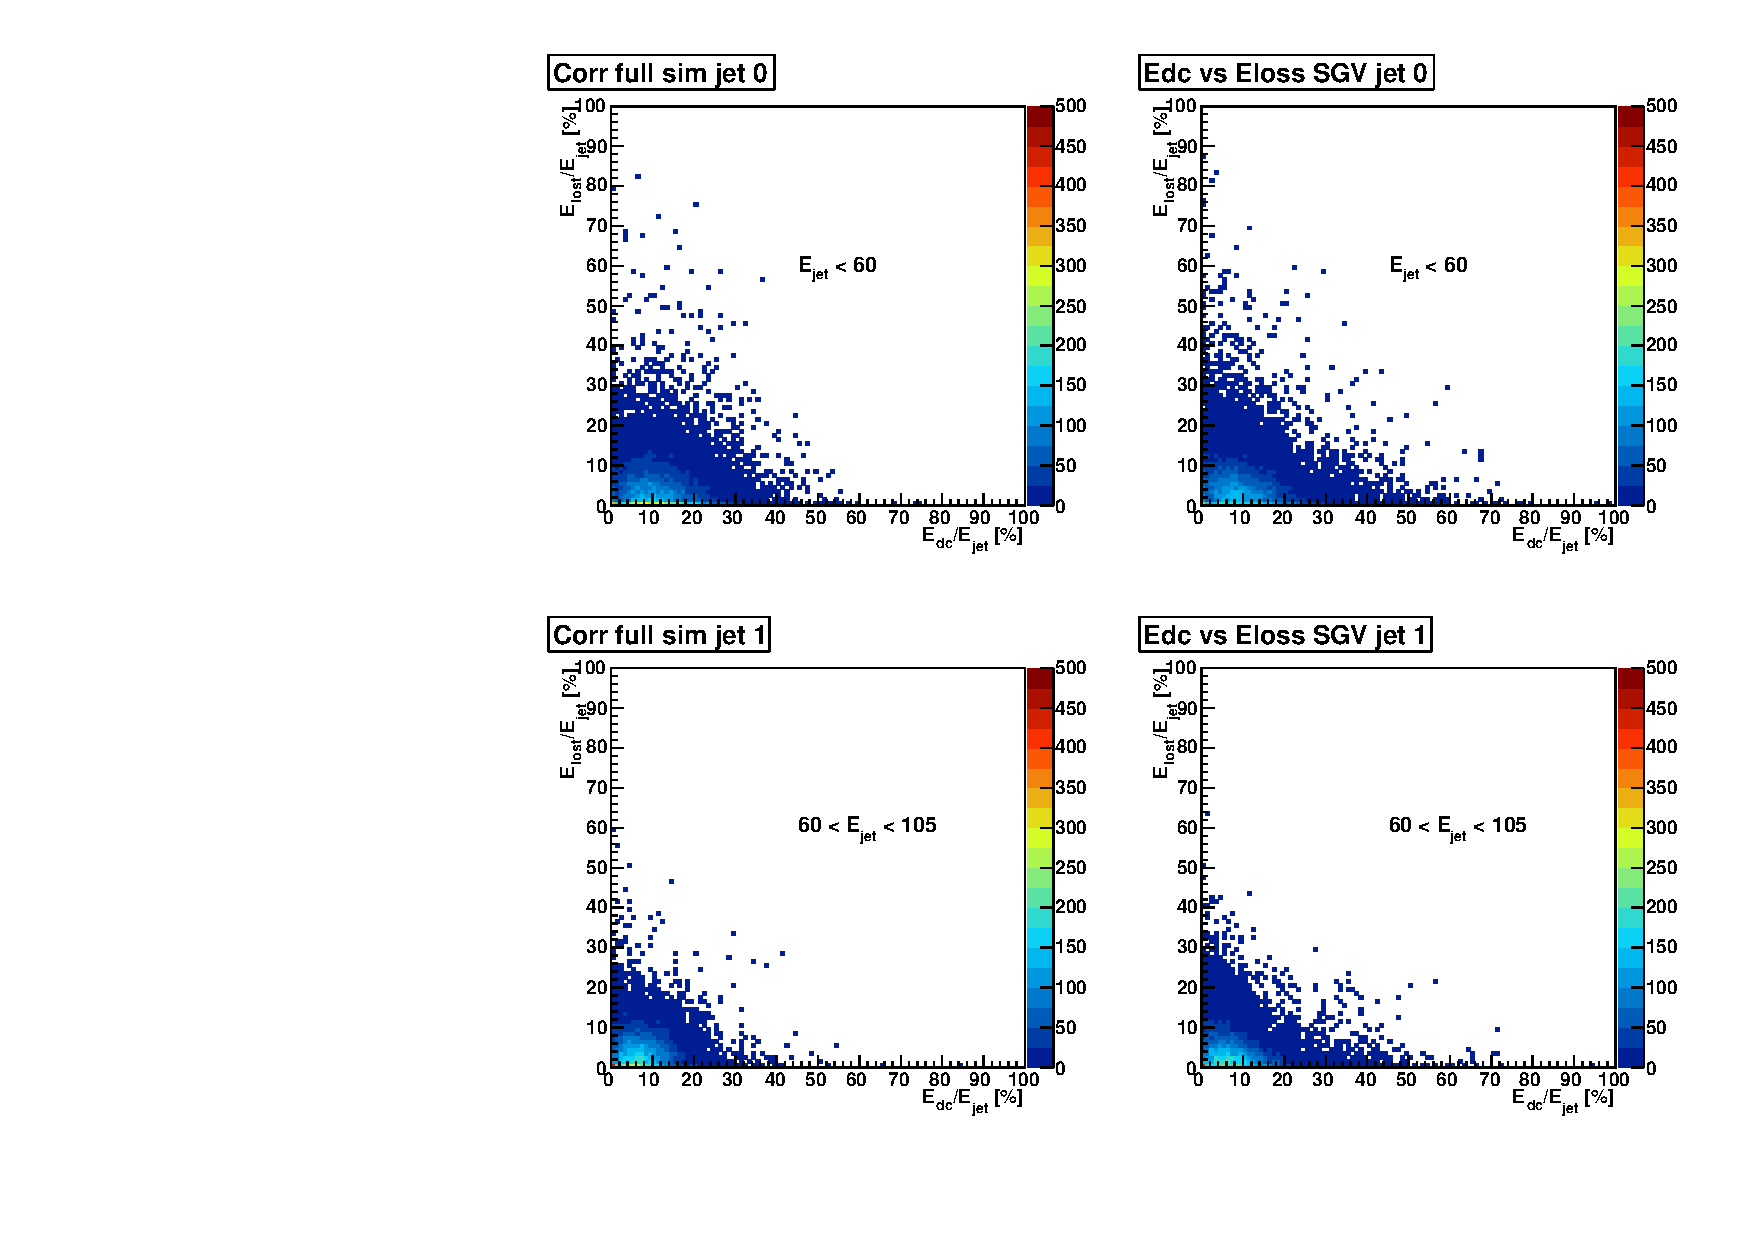
\includegraphics[width=1\linewidth]{chap6/fig_SGV/Correlation_1.pdf}
    \caption{} \label{fig:jet_track_level_full}
  \end{subfigure}
  \hfill
  \begin{subfigure}[t]{0.45\textwidth}
    \centering
    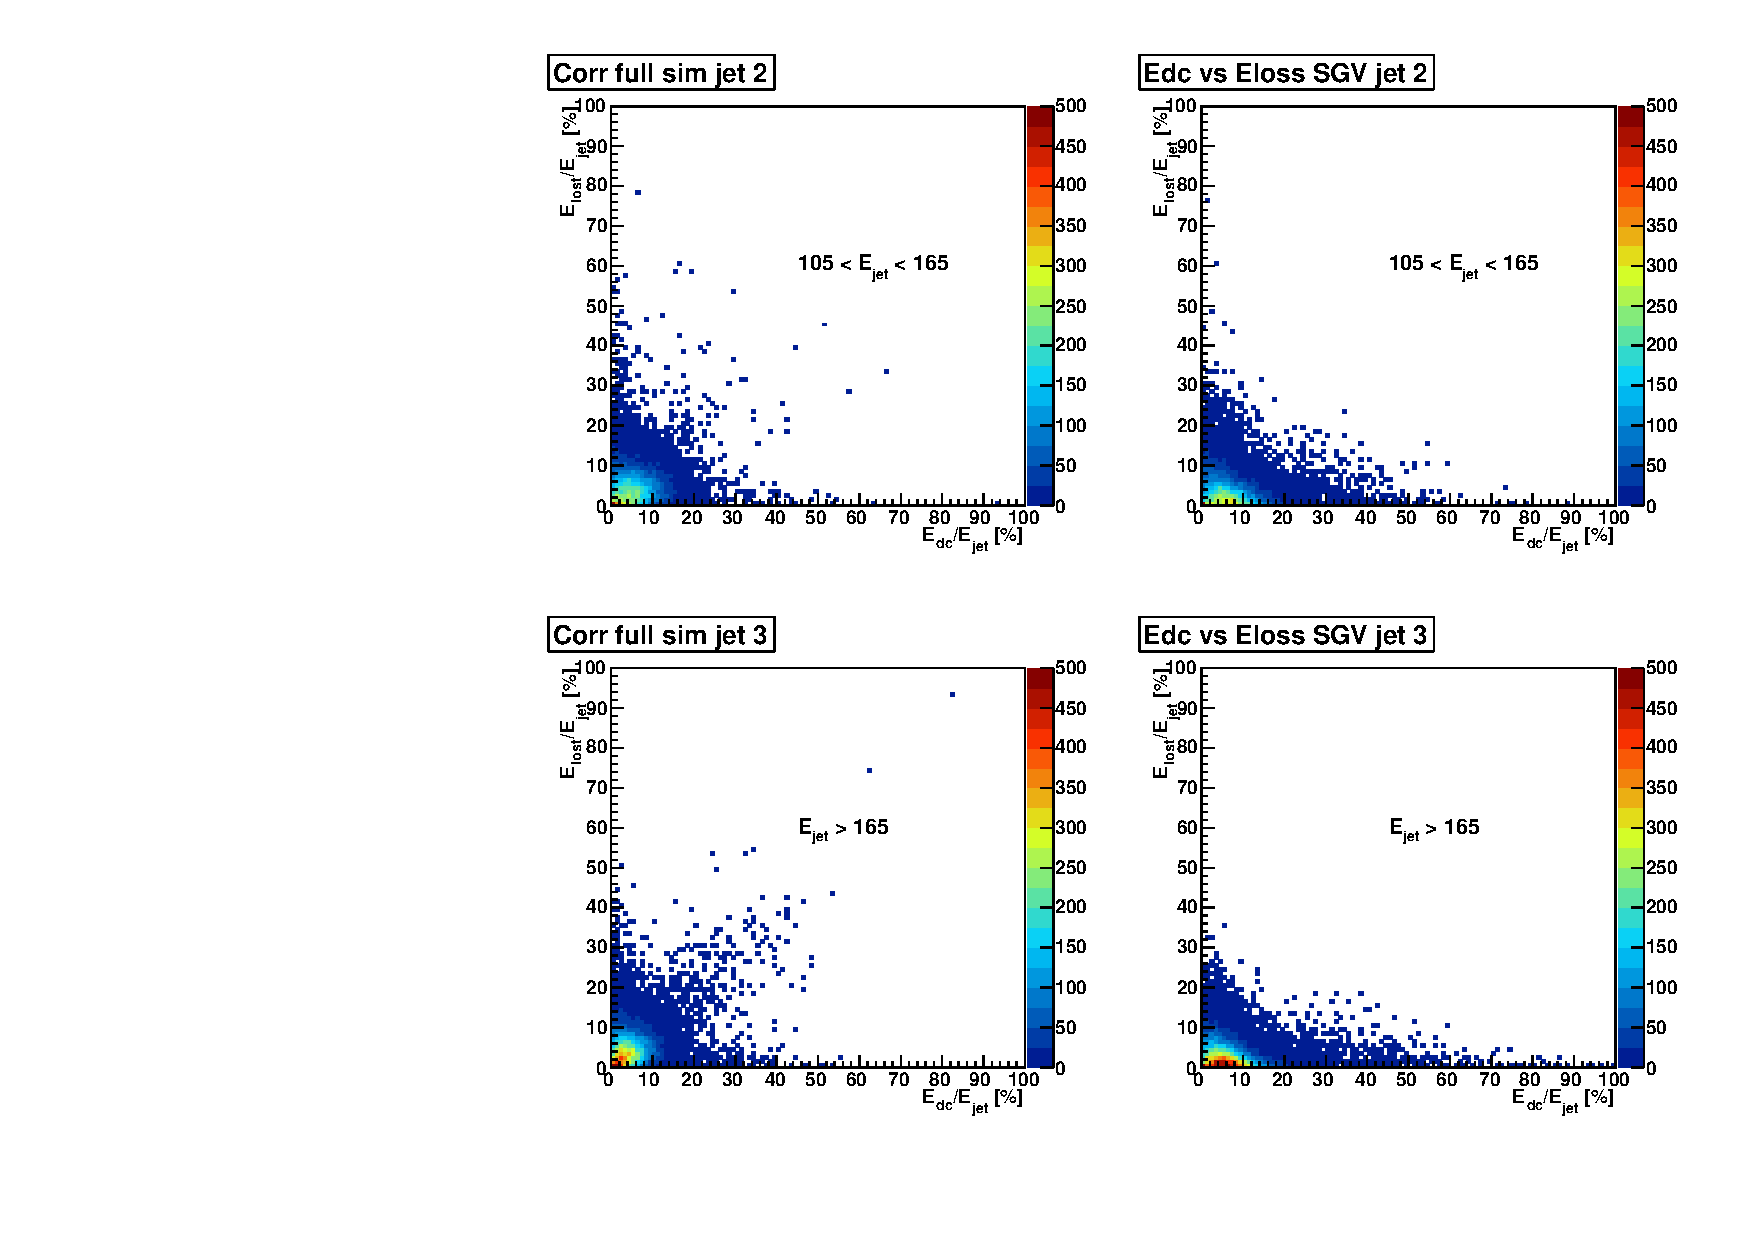
\includegraphics[width=1\linewidth]{chap6/fig_SGV/Correlation_2.pdf}
    \caption{} \label{fig:jet_track_level_sgv}
  \end{subfigure}
  \caption{\subref{fig:jet_track_level_full}) Correlation between $E_{lost}$ and $E_{dc}$ for the full simulation. \subref{fig:jet_track_level_sgv}) Correlation between $E_{lost}$ and $E_{dc}$ for SGV fast simulation.}
\end{figure}

This may indicate that the current parametrisation can be improved and that the merging and splitting probabilities should be then function of the energy density in the calorimeter region studied.

\subsection{Energy fraction inside a jet}

Jets are composed of many charged and neutral particles. For each jet energy bin, the distribution of the charged/neutral energy fraction to the jet energy was looked at. It could give a handle in order to understand the effect of the parametrisation on a jet level and the observed discrepencies between the full simulation and SGV.

\begin{figure}[t]
  \centering
  \begin{subfigure}[t]{0.45\textwidth}
    \centering
    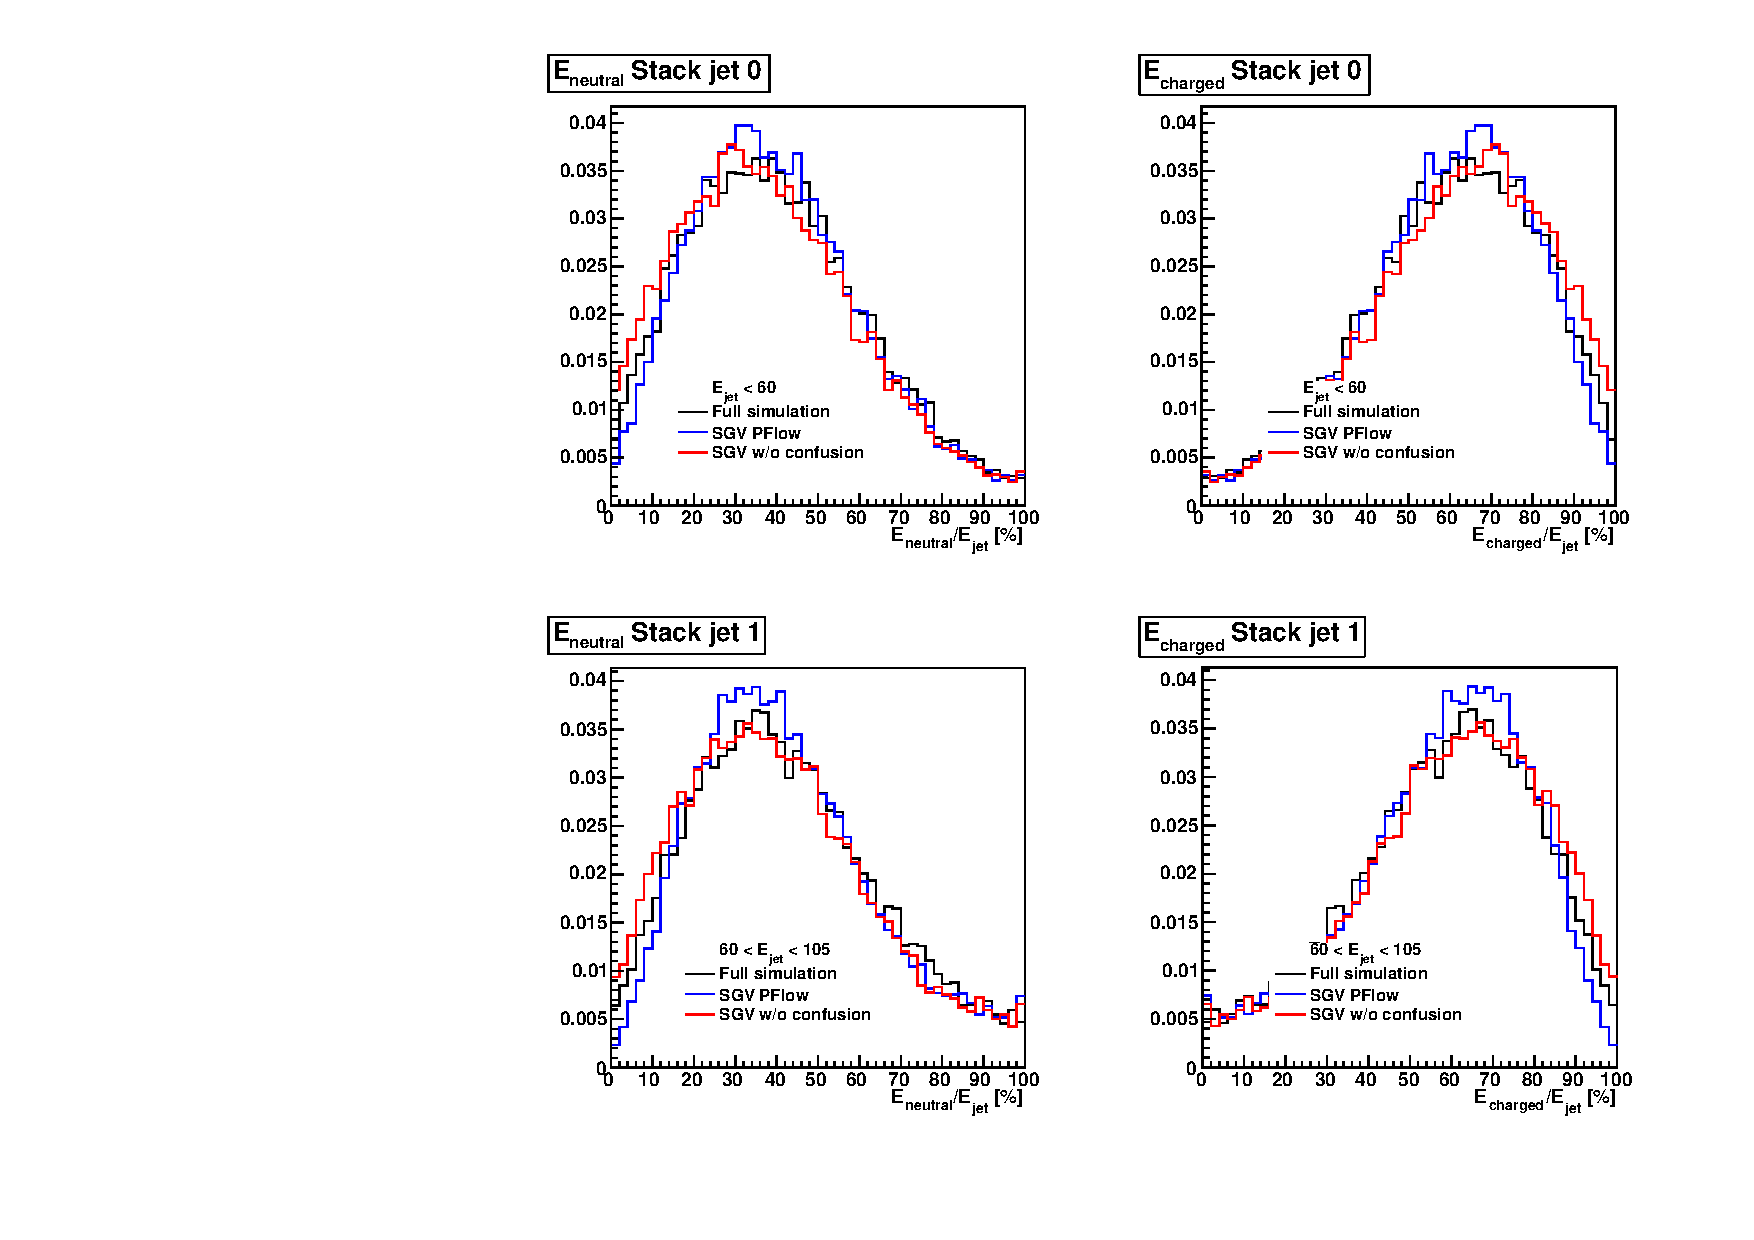
\includegraphics[width=1\linewidth]{chap6/fig_SGV/EneuEcha_binned_1.pdf}
    \caption{Energy distribution for charged and neutrals normalised to the jet energy for bin 1 and 2 of jet energy.} \label{fig:jet_track_level_bins12}
  \end{subfigure}
  \hfill
  \begin{subfigure}[t]{0.45\textwidth}
    \centering
    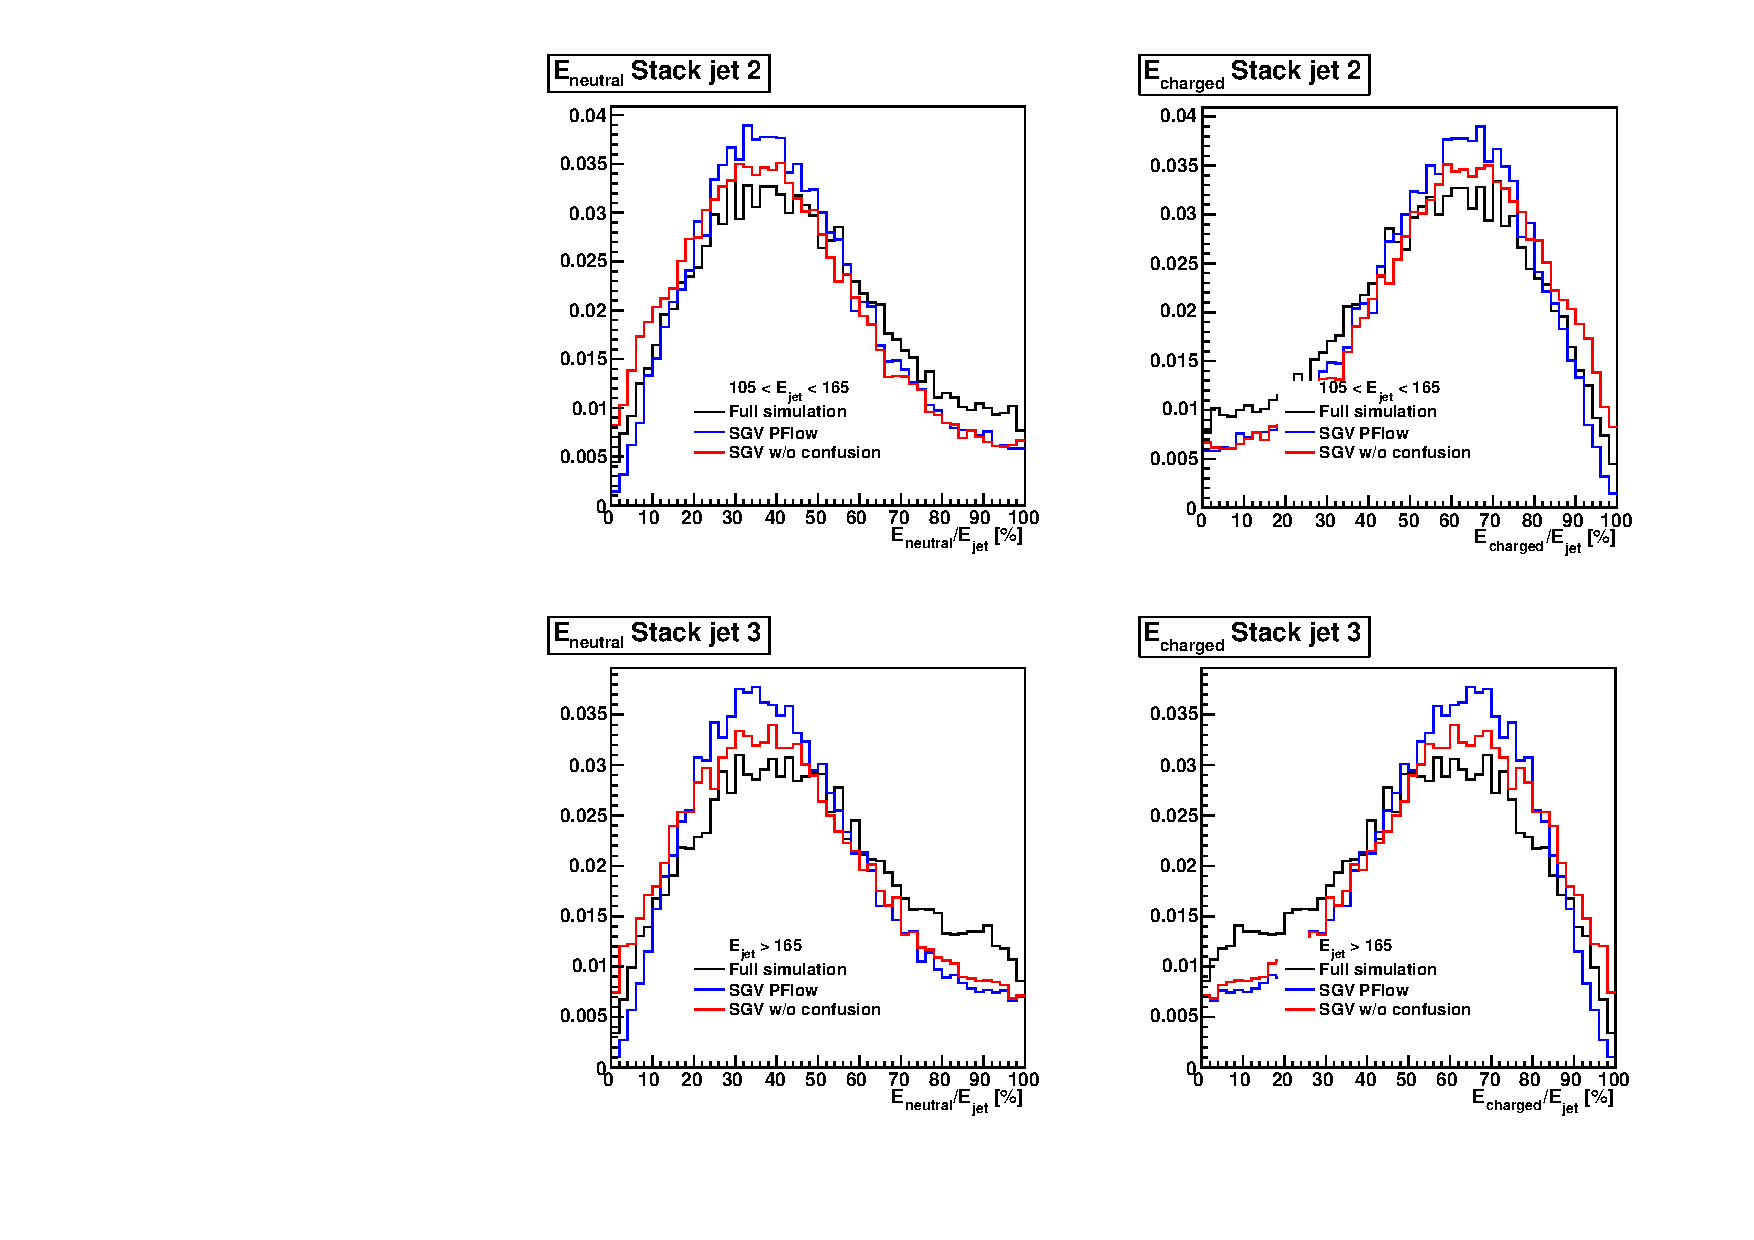
\includegraphics[width=1\linewidth]{chap6/fig_SGV/EneuEcha_binned_2.pdf}
    \caption{Energy distribution for charged and neutrals normalised to the jet energy for bin 3 and 4 of jet energy.} \label{fig:jet_track_level_bins34}
  \end{subfigure}
  \caption{\subref{fig:jet_track_level_bins12}) Energy distribution for charged and neutrals normalised to the jet energy under 105 \GeV. The black line represents the full simulation, the red/blue line represents SGV fast simulation. \subref{fig:jet_track_level_bins34}) Energy distribution for charged and neutrals normalised to the jet energy over 105 \GeV. The black line represents the full simulation, the red/blue line represents SGV fast simulation.}
\end{figure}

For the energy distribution on figures \ref{fig:jet_track_level_bins12} and \ref{fig:jet_track_level_bins34}, one can observe that the plots of neutral and charged energy are mirror to each other, as the sum of the charged and neutral energy should be equal to the jet energy. For low energy jets, the distributions seems to be rather in a good agreement, only small discrepancies are visible in the low/high fraction regions. For higher jet energies, this discrepancy is getting bigger. There is more neutral energy in the 50-70\% region and much less in the 10-20\% region for charged particles. Somehow SGV is pulling the energy in the wrong direction by splitting too much charged clusters.

The idea is that charged energy from the 50+\% region should be transferred to the 10-20\% region, meaning that charged clusters are transformed to neutral clusters. That is how the total charged energy distribution could be shifted toward lower energies by \"losing\" charged energy and gaining neutral energy. This is consistent with the assumption that PandoraPFA is switching to an \"Energy flow\" mode. It can occurs during this process that charged cluster are transformed to neutral cluster in order to match the $E/p$ locally. PandoraPFA only takes care of the calorimeter information and discards the track information.

\subsection{Occupancy and Energy density}

One relative variable in the splitting and merging probabilities is the distance between a cluster of one type (hadronic or electromagnetic) and a cluster of the other type. The study of the distribution of the distance to the nearest neighbour was performed distinguishing between ECAL and HCAL, basically electromagnetic and hadronic showers.

The procedure is perform such as in each jet, a list of neutral and charged particles is filled. Each of theses particles are projected either on the barrel or the endcap of the ECAL or HCAL depending on the nature of the cluster (EM or hadronic). The projection is done in order to calculate distances on the same geometry planes as SGV and the full simulation have slight different geometries. For neutrals, a simple calculation is done assuming a propagation at the speed of light. The intersection is calculated at the ECAL/HCAL endcap front face ($z_{ECAL} = 2450 mm$ / $z_{HCAL} = 2650 mm$) or ECAL/HCAL barrel front face ($r_{ECAL} = 1843 mm$ / $r_{HCAL} = 2058 mm$) according to ILD geometry as described in section \ref{}. For charged, the \lcio track is propagated following the helix parametrisation until the front face of the ECAL/HCAL in the endcap or barrel.

After this, the list of neutrals is looped over and the distance to all charged particles:
\begin{equation}
  r_{ij} = \sqrt{(x_i - x_j)^2 + (y_i - y_j)^2 + (z_i - z_j)^2}
\end{equation}
with $x_{i,j}$, $y_{i,j}$, $z_{i,j}$ the coordinates of the neutral particle $i$ and any charged particle $j$ at the front face of the ECAL/HCAL is calculated. A distinction between endcap and barrel is done to get rid of corner effects. The minimum distance $d_{min}$ is defined as $min(r_{ij})$ for each neutral particle. The plots are shown on figures \ref{fig:dmin_ECAL} and \ref{fig:dmin_HCAL}.

\begin{figure}[t]
  \centering
  \begin{subfigure}[t]{0.45\textwidth}
    \centering
    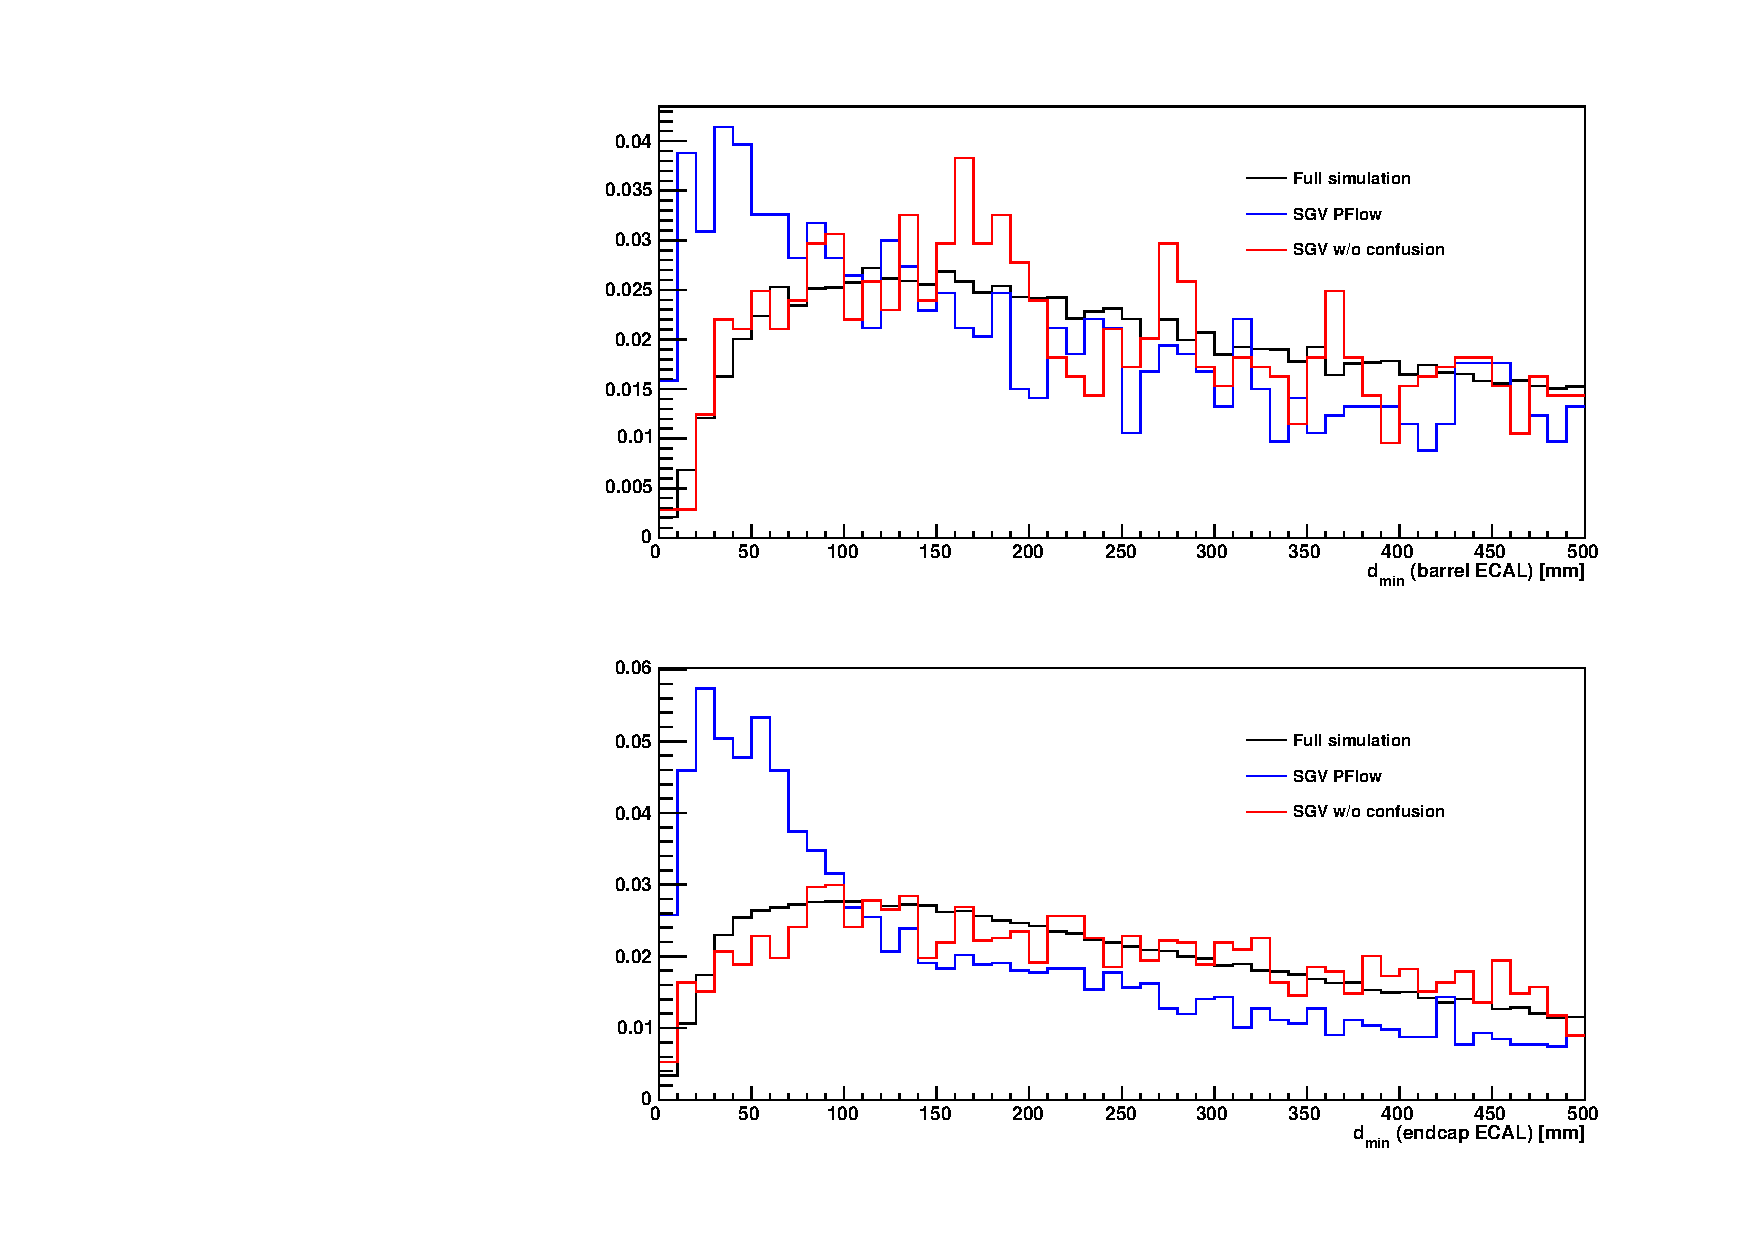
\includegraphics[width=1\linewidth]{chap6/fig_SGV/dmin_charged_to_neutral_ECAL_all.pdf}
    \caption{ECAL case.} \label{fig:dmin_ECAL}
  \end{subfigure}
  \hfill
  \begin{subfigure}[t]{0.45\textwidth}
    \centering
    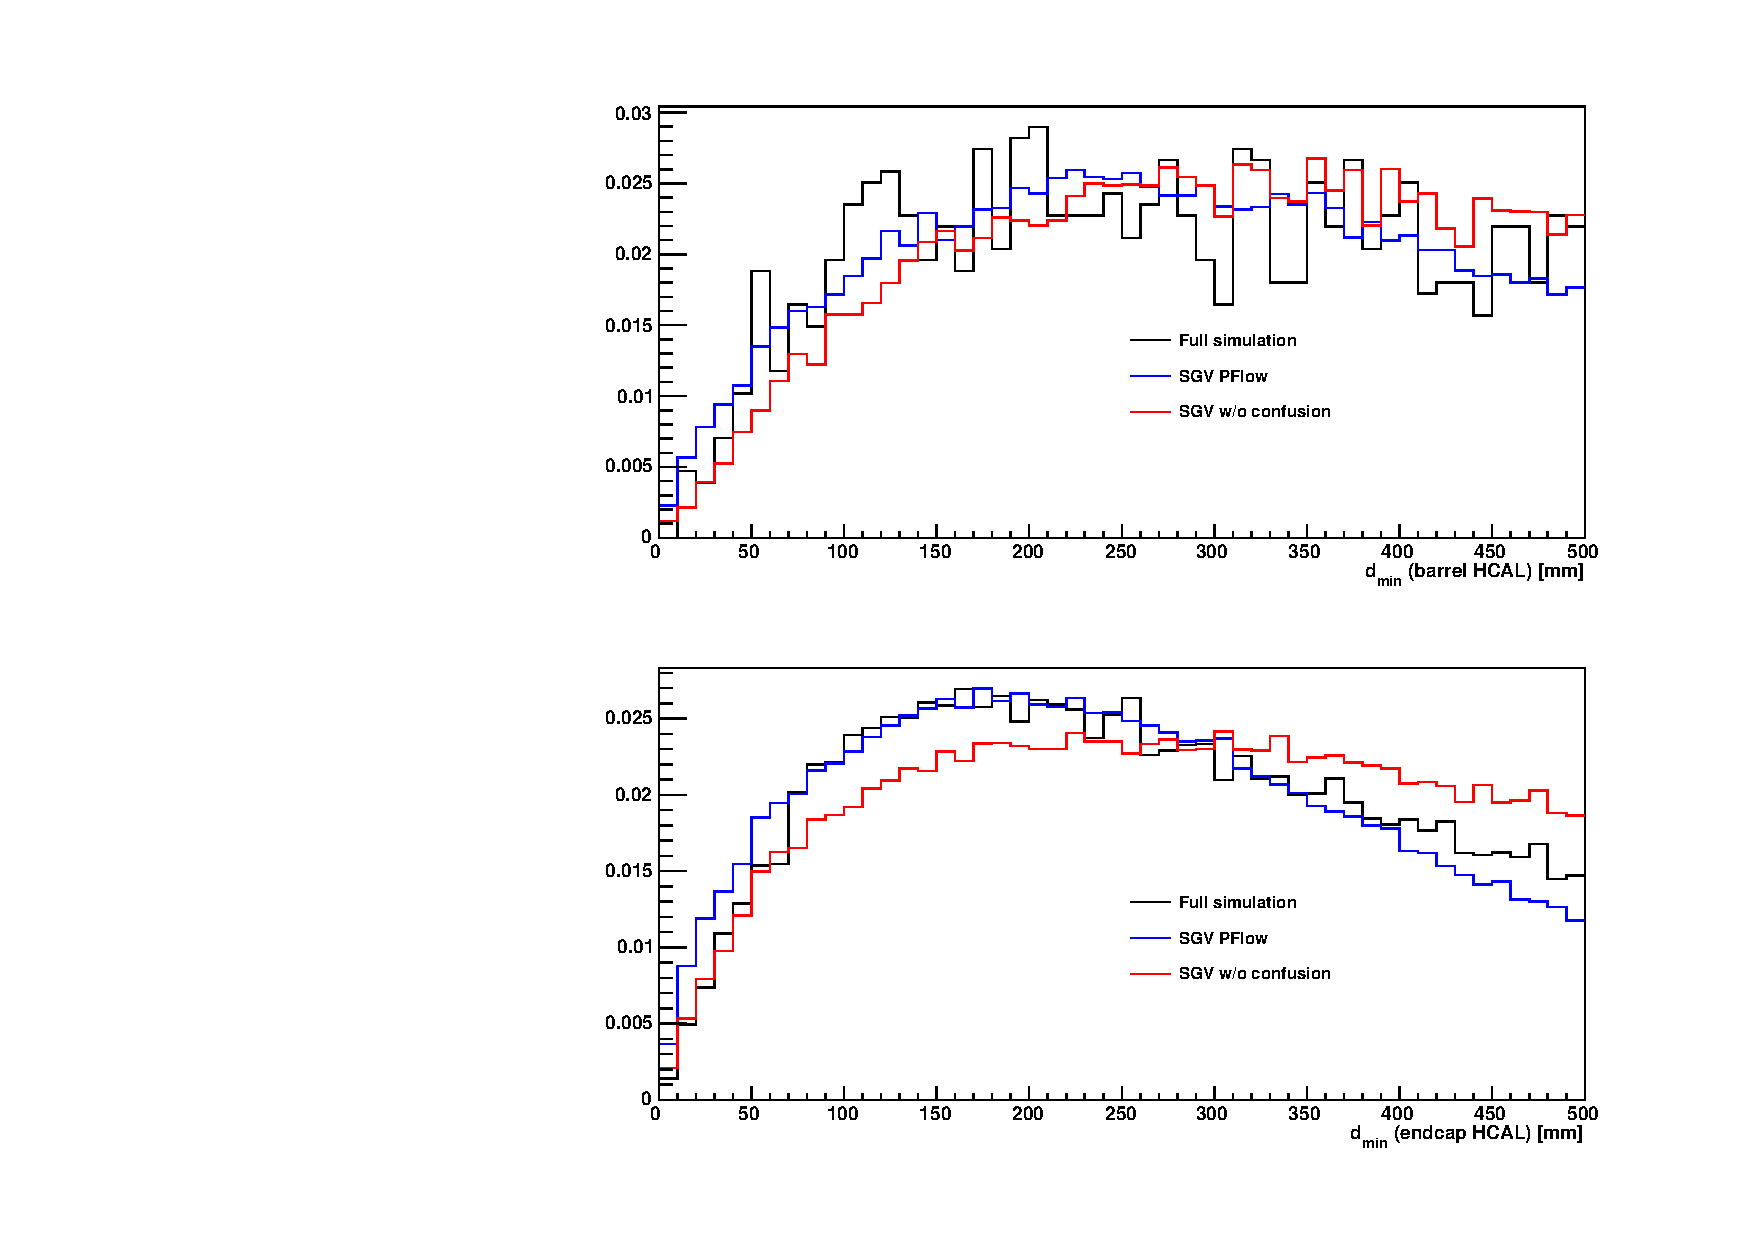
\includegraphics[width=1\linewidth]{chap6/fig_SGV/dmin_charged_to_neutral_HCAL_all.pdf}
    \caption{HCAL case.} \label{fig:dmin_HCAL}
  \end{subfigure}
  \caption{\subref{fig:dmin_ECAL}) Distance neutral to the closest charged distribution for the ECAL. \subref{fig:dmin_HCAL}) Distance neutral to the closest charged distribution for the HCAL.}
\end{figure}

One can observe that there is a discrepancy between full simulation and SGV with Particle Flow in the ECAL. The Particle Flow parametrisation seems to have the effect that particles are placed closer in the ECAL. On the other hand, the Particle Flow parametrisation seems to have a rather good effect in the HCAL. Thus the PFA parametrisation was disable for the ECAL and the same distributions were looked again as shown on figures \ref{fig:dmin_ECAL_noPFA} and \ref{fig:dmin_HCAL_noPFA}.

% \begin{figure}[t]
%   \centering
%   \begin{subfigure}[t]{0.45\textwidth}
%     \centering
%     \includegraphics[width=1\linewidth]{chap6/fig_SGV/dmin_ECAL_2.pdf}
%     \caption{.} \label{fig:dmin_ECAL_noPFA}
%   \end{subfigure}
%   \hfill
%   \begin{subfigure}[t]{0.45\textwidth}
%     \centering
%     \includegraphics[width=1\linewidth]{chap6/fig_SGV/dmin_HCAL_2.pdf}
%     \caption{.} \label{fig:dmin_22}
%   \end{subfigure}
%   \caption{\subref{fig:dmin_2}) . \subref{fig:dmin_HCAL_noPFA}) .}
% \end{figure}

% \captionof{figure}{Distance to the closest charged distribution for the ECAL with Particle Flow parametrisation disable on the left and the HCAL on the right.}

In that case, the distributions are in rather good agreement for the ECAL and HCAL. The Particle Flow parametrisation seems to have a rather limited effect on the ECAL distribution compared to SGV without Particle Flow.

Is the parametrisation of Particle Flow in SGV useless for the ECAL? In order to check the influence of the parametrisation on the ECAL energy distribution, the charged and neutral energy were looked at again. As expected, switching off the Particle Flow parametrisation for the ECAL have rather no or limited impact on the charged energy distribution as shown on figure \ref{fig:energy_ECALnoPFA}.

\begin{figure}[t]
  \centering
  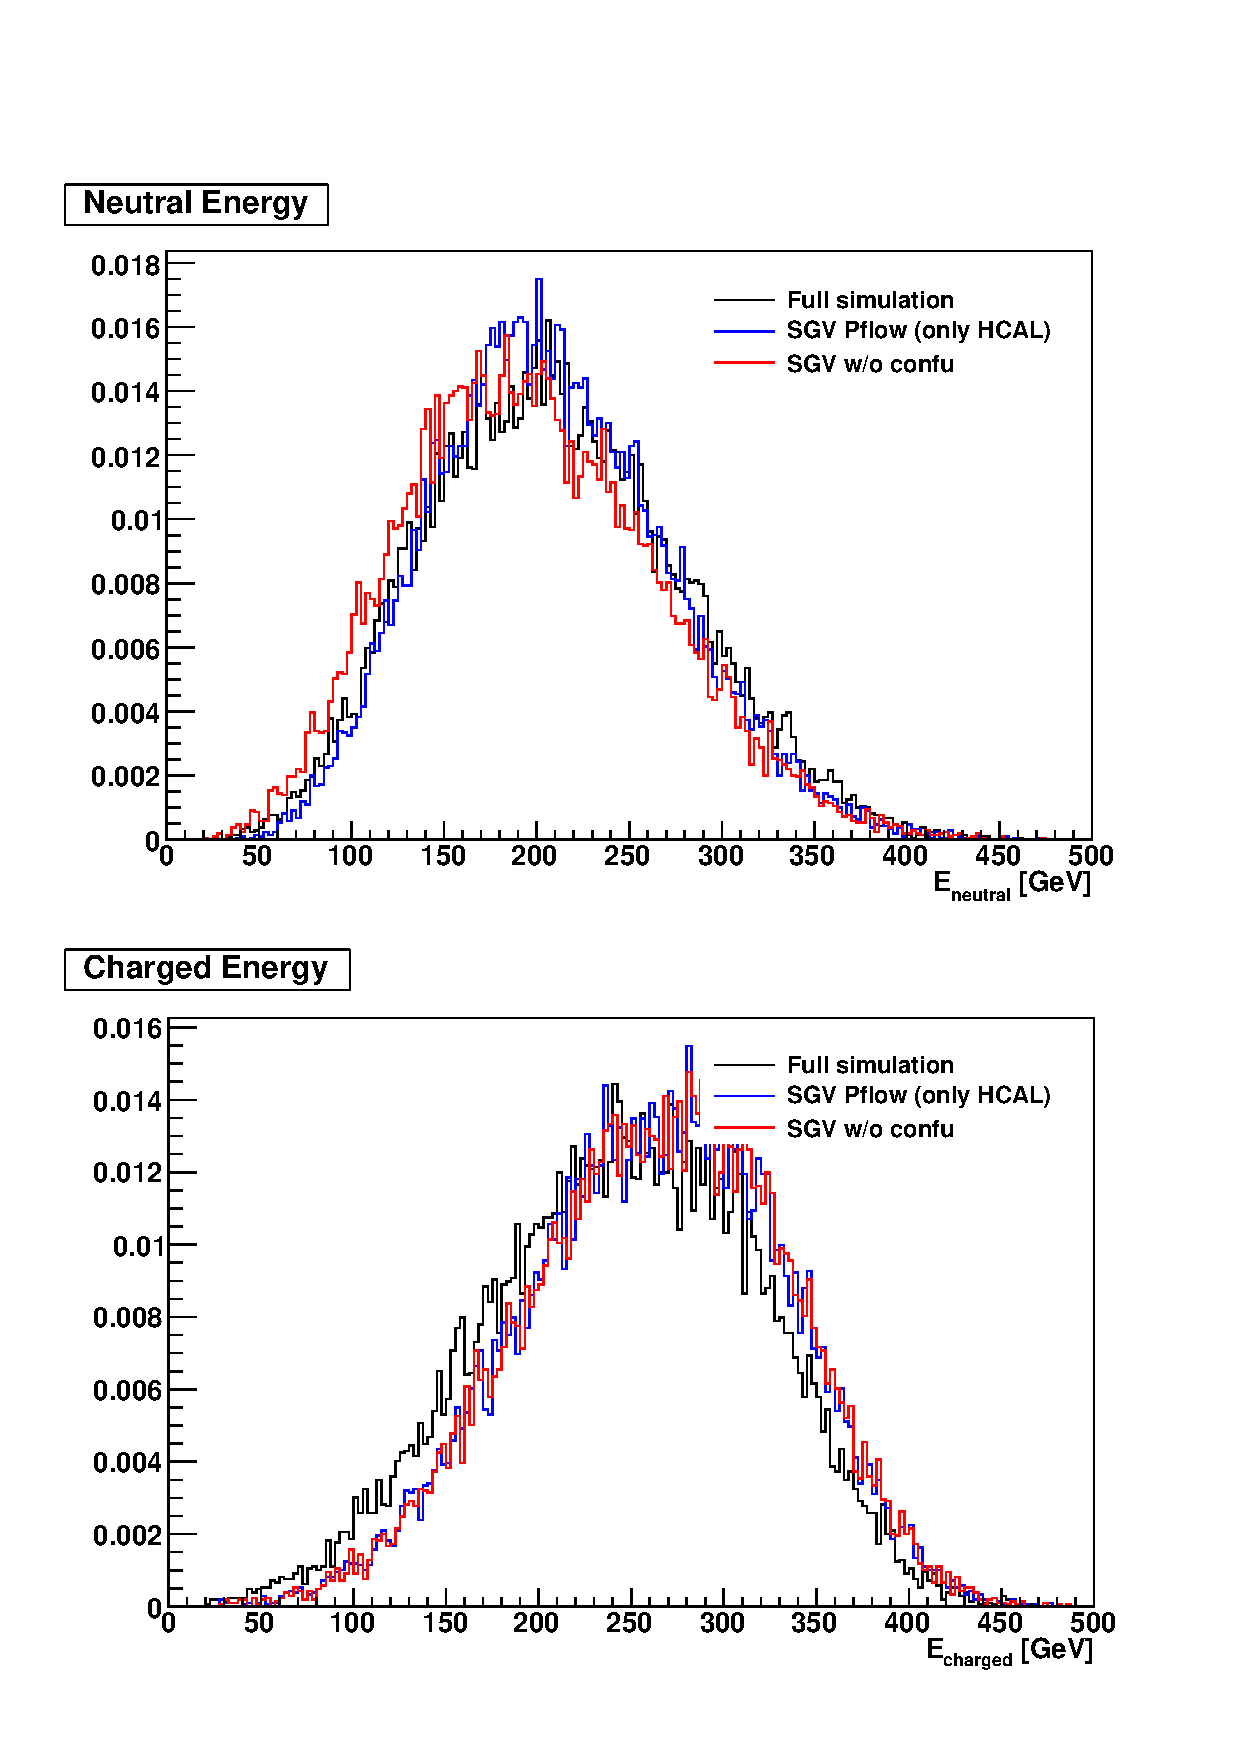
\includegraphics[width=1\linewidth]{chap6/fig_SGV/Total_EneuEcha_notjet_onlyHCAL.pdf}
  \caption{Neutral and charged energy distributions with Particle Flow disabled for the ECAL.}
  \label{fig:energy_ECALnoPFA}
\end{figure}

One variable to look at would be the occupancy of the detector in the jet region or the energy density. This is could give us a clue to understand how PandoraPFA is splitting and merging in function of the energy density and then implement or correct the splitting and merging probabilities used in SGV to parametrise Particle Flow.

\section{Conclusion}

In conclusion, the benchmark of the fast simulation SGV was done. A Particle Flow parametrisation is implemented in SGV and most of the results obtained are in agreement with the full simulation. Still the parametrisation is not perfectly correct as there is still some discrepancies between SGV and the full simulation (Total energy, distance to the nearest neighbour, correlation between $E_{dc}$ and $E_{lost}$...).

The next steps would be to look at the energy density distribution in a jet region and parametrise the splitting and merging probabilities of a cluster in function of the density and achieve an even better agreement between SGV and the full simulation.
